\documentclass[11pt]{article}
\usepackage[a4paper,margin=1in]{geometry}
\usepackage{lmodern}
\usepackage[T1]{fontenc}
\usepackage{microtype}
\usepackage{amsmath,amssymb,amsthm,bm}
\usepackage{mathtools}
\usepackage{booktabs}
\usepackage{enumitem}
\usepackage{hyperref}
\usepackage{cleveref}
\usepackage{algorithm}
\usepackage{algpseudocode}
\usepackage{tikz}
\usetikzlibrary{arrows.meta,positioning,calc,fit,shapes.misc,shapes.geometric, calc, bayesnet}
% \usetikzlibrary{bayesnet, arrows, positioning, fit, shapes.geometric}
\newcommand{\vecs}[1]{\boldsymbol{#1}} % For vectors, e.g., alpha, mu
\theoremstyle{definition}
\newtheorem{definition}{Definition}
\newtheorem{proposition}{Proposition}
\newtheorem{remark}{Remark}
\newtheorem{lemma}{Lemma}
\newcommand{\Feedback}{\mathsf{Feedback}}
\title{Learning to Defer For Time Series via Switching State-Space Models}
\author{}
\date{\today}

\newcommand{\E}{\mathbb{E}}
\newcommand{\Var}{\mathrm{Var}}
\newcommand{\Cov}{\mathrm{Cov}}
\newcommand{\1}{\mathbf{1}}
\newcommand{\R}{\mathbb{R}}
\newcommand{\given}{\,\middle|\,}
\newcommand{\Normal}{\mathcal{N}}
\newcommand{\N}{\mathbb{N}}
\newcommand{\I}{\mathcal{I}}  % Information set
\newcommand{\Regime}{\mathcal{Z}} % Regime space
\newcommand{\Expert}{\mathcal{K}} % Expert set
\newcommand{\trans}{^{\top}}


\newcommand{\bmalpha}{\vecs{\alpha}}
\newcommand{\bmSigma}{\vecs{\Sigma}}
\newcommand{\bmK}{\vecs{K}}

\begin{document}
\maketitle




\begin{abstract}
We present a theoretical framework for Learning-to-Defer (L2D) in non-stationary time series environments where querying experts incurs an explicit consultation cost. We formalize the problem as a sequential decision process under partial observation with a time-varying set of experts. We model the time-varying reliability of black-box experts (e.g., neural networks) as latent states in a Switching Linear Dynamical System (SLDS). This structure captures abrupt environmental shifts (regimes) and gradual performance drift. We derive a tractable inference algorithm using the Interacting Multiple Model (IMM) filter, providing full derivations for the variance spread in Gaussian mixtures, and propose a cost-sensitive myopic selection policy that balances predictive risk, epistemic uncertainty, and operational costs.
\end{abstract}

Note: might be interested to predict when the expert will be or not available?

\section{Problem Formulation}

\subsection{Preliminaries}

We consider a sequential forecasting and routing problem over a discrete horizon
$t=1,\dots,T$. All random quantities are defined on a probability space
$(\Omega,\mathcal{F},\mathbb{P})$ equipped with a \emph{pre-decision} filtration
$\mathbb{F}=\{\mathcal{F}_t\}_{t\ge 0}$.
Here, $\mathcal{F}_t$ represents the information available to the router \emph{at decision time} $t$,
i.e., immediately \emph{before} selecting an expert at time $t$.

\paragraph{Static randomness and expert labels.}
We let $\mathcal{F}_0$ encode any static randomness (e.g., unknown model parameters and/or the collection of expert prediction
rules), and assume $\mathcal{F}_0$ is independent of the online evolution unless stated otherwise.
We assume all experts carry unique labels in a common (finite or countable) universe $\mathcal U$ (e.g., $\mathcal U=\mathbb{N}$),
so that all expert indices take values in the same measurable space.

\begin{itemize}
    \item \textbf{Context and target (regression setting).}
    At each time $t$, nature reveals a context vector $\mathbf{x}_t \in \mathcal{X}\subseteq\mathbb{R}^d$.
    The router observes $\mathbf{x}_t$ at decision time, so $\mathbf{x}_t$ is $\mathcal{F}_t$-measurable.
    The associated ground-truth target is
    \[
        y_t \in \mathcal{Y}\subseteq\mathbb{R},
    \]
    which is \emph{not} observed at decision time; in particular, $y_t$ need not be $\mathcal{F}_t$-measurable.

    \item \textbf{Dynamic expert registry (the roster).}
    Let $\mathcal{U}_t\subseteq \mathcal U$ denote the \emph{registry} of all experts encountered up to time $t$.
    The registry evolves cumulatively to preserve the learned history of temporarily unavailable experts:
    \[
        \mathcal{U}_t \coloneqq \mathcal{U}_{t-1} \cup \Expert_t
        \qquad (\text{with } \mathcal{U}_0 = \varnothing).
    \]

    \item \textbf{Expert availability.}
    At decision time $t$, only a subset $\Expert_t \subseteq \mathcal{U}_t$ is available for querying.
    We assume $\Expert_t$ is observed at decision time (hence $\mathcal{F}_t$-measurable) and
    \[
        \mathbb{P}(\Expert_t \neq \varnothing)=1
        \qquad \text{for all } t=1,\dots,T.
    \]

    \item \textbf{Expert predictions.}
    Each expert $j\in\mathcal U$ is associated with a prediction rule
    $f_j:\mathcal{X}\to\mathcal{Y}$, which is either deterministic or, more generally, $\mathcal{F}_0$-measurable and fixed over time.
    If $j\in\Expert_t$, then at time $t$ expert $j$ returns
    \[
        \hat{y}_t^{(j)} \coloneqq f_j(\mathbf{x}_t).
    \]

    \item \textbf{Latent regimes and cross-expert dependence (modeling scope).}
    Our generative model (introduced later) includes a latent regime process $(z_t)_{t\ge1}$ and a shared latent factor
    $(g_t)_{t\ge1}$ that can induce \emph{correlations across experts} at a fixed time~$t$.
    Accordingly, we do \emph{not} assume the losses $(\ell_{j,t})_{j\in\mathcal{U}_t}$ are independent across $j$.
    We may allow regime transitions to depend on contexts (``context-dependent switching''); when presenting specific inference/learning procedures later,
    we will state explicitly whether transitions are treated as time-homogeneous or input-driven.

    \item \textbf{Loss process and bandit (censored) feedback.}
    Performance is evaluated through a loss function
    \[
        \mathcal{L}:\mathcal{Y}\times\mathcal{Y}\to[0,+\infty).
    \]
    The (counterfactual) instantaneous loss of expert $j$ at time $t$ is the random variable
    \[
        \ell_{j,t} \coloneqq \mathcal{L}\!\bigl(\hat{y}_t^{(j)},y_t\bigr)\in[0,+\infty).
    \]
    Under bandit (censored) feedback, once the router selects $r_t\in\Expert_t$ at time $t$,
    it observes only the realized loss $\ell_{r_t,t}$, while $\{\ell_{j,t}:j\neq r_t\}$ remain unobserved.
    The observed loss is revealed \emph{after} the decision at time $t$ and is available to the router at the next decision time,
    i.e., it becomes $\mathcal{F}_{t+1}$-measurable.

    \item \textbf{History and admissible policies.}
    Define the end-of-round feedback random element
    \[
        G_t \coloneqq (r_t,\ell_{r_t,t}) \in \mathcal U\times[0,+\infty).
    \]
    The interaction history available at decision time $t$ (i.e., up to round $t-1$) is
    \[
        \mathcal{I}_{t-1} \coloneqq \bigl((\mathbf{x}_\tau,\Expert_\tau,G_\tau)\bigr)_{1\le \tau \le t-1},
        \qquad \mathcal{I}_0 \text{ empty}.
    \]
    The information available at decision time $t$ is summarized by
    \[
        H_t \coloneqq (\mathcal{I}_{t-1},\mathbf{x}_t,\Expert_t).
    \]
    We take the pre-decision filtration to be generated by this information together with the static sigma-field:
    \[
        \mathcal{F}_t \coloneqq \sigma(H_t)\vee \mathcal{F}_0, \qquad t=1,\dots,T.
    \]
    A (deterministic) routing policy is a sequence of measurable maps
    \[
        \pi_t:\mathsf{H}_t\to\mathcal U, \qquad t=1,\dots,T,
    \]
    where $\mathsf{H}_t$ denotes the measurable space in which $H_t$ takes values, such that
    $\pi_t(H_t)\in\Expert_t$ almost surely.
    The chosen expert at time $t$ is
    \[
        r_t \coloneqq \pi_t(H_t),
    \]
    and in particular $r_t$ is $\mathcal{F}_t$-measurable with values in $\Expert_t$ almost surely.
\end{itemize}

\paragraph{Running Example (Medical Triage).}
Consider an automated triage system in a hospital Emergency Room.
\begin{itemize}
    \item The \textbf{Context} $\mathbf{x}_t$ represents a patient's initial vitals, laboratory values, and presenting symptoms.
    \item The \textbf{Target} $y_t$ is a real-valued outcome, e.g., a risk score or a biomarker observed after further testing.
    \item The \textbf{Experts} in $\Expert_t$ are diagnostic models or human specialists currently available (e.g., an on-call cardiologist).
          The set $\Expert_t$ varies over time. The system maintains a \textbf{registry} $\mathcal{U}_t$ to track all specialists encountered so far,
          including those currently off-duty, allowing for immediate calibrated use upon their return.
    \item The \textbf{Loss} $\ell_{j,t}$ quantifies discrepancy between $f_j(\mathbf{x}_t)$ and $y_t$ (e.g., squared error).
          Only $\ell_{r_t,t}$ for the selected expert $r_t$ is observed and enters future decisions.
    \item \textbf{Non-stationarity} can arise from distribution shifts and/or latent regime switches (potentially influenced by the observed context).
\end{itemize}
The router must therefore select at each time $t$ an expert $r_t\in\Expert_t$ using only $(\mathbf{x}_t,\Expert_t)$ and the past history $\mathcal{I}_{t-1}$,
without observing $y_t$ (or the full loss vector $(\ell_{j,t})_{j\in\mathcal{U}_t}$) at decision time.

\subsection{The Decision Process}

The system operates as a \emph{cost-sensitive router}.
At each decision epoch $t\in\{1,\dots,T\}$, after observing
\[
    H_t = (\mathcal I_{t-1},\mathbf x_t,\Expert_t),
\]
the router selects a single expert index $r_t\in \Expert_t$ to query.

\begin{itemize}
    \item \textbf{Action space.}
    The admissible actions at time $t$ are exactly the currently available experts,
    i.e.\ the finite set $\Expert_t \subseteq \mathcal{U}_t \subseteq \mathcal U$:
    \[
        r_t \in \Expert_t.
    \]

    \item \textbf{Consultation costs.}
    Each expert $j\in\mathcal U$ is associated with a deterministic, nonnegative consultation cost
    \[
        \beta_j \ge 0,
    \]
    modeling, e.g., API fees, latency, computational/energy cost, or operational constraints.
    The costs $(\beta_j)_{j\in\mathcal{U}_t}$ are assumed known for all registered experts
    (persisting in memory even when experts are temporarily unavailable/offline).
\end{itemize}

\paragraph{Realized cost.}
Given an action $r_t\in\Expert_t$, the \emph{total realized cost} at time $t$ is
\begin{equation}\label{eq:realized_cost}
    C_t(r_t)
    \;\coloneqq\;
    \underbrace{\ell_{r_t,t}}_{\text{prediction loss}}
    \;+\;
    \underbrace{\beta_{r_t}}_{\text{consultation cost}}.
\end{equation}
At decision time $t$, $\beta_{r_t}$ is known, whereas $\ell_{r_t,t}$ is random.
Under bandit feedback, $\ell_{r_t,t}$ is revealed only after taking the action and is incorporated into the next decision
via the updated history $\mathcal I_t$ (hence it is $\mathcal F_{t+1}$-measurable).

\paragraph{Objective.}
A (deterministic, possibly non-stationary) policy is a measurable sequence
$\pi=(\pi_t)_{t=1}^T$ such that $\pi_t(H_t)\in\Expert_t$ almost surely; the action is
$r_t \coloneqq \pi_t(H_t)$.
The goal is to minimize the expected cumulative cost over the horizon:
\begin{equation}
    \label{eq:objective}
    \inf_{\pi}
    \;
    \mathbb{E}
    \left[
        \sum_{t=1}^T C_t\bigl(\pi_t(H_t)\bigr)
    \right]
    \;=\;
    \inf_{\pi}
    \;
    \mathbb{E}
    \left[
        \sum_{t=1}^T
        \Bigl(
            \ell_{\pi_t(H_t),t}
            + \beta_{\pi_t(H_t)}
        \Bigr)
    \right].
\end{equation}

\paragraph{POMDP formulation (latent state and information state).}
To make explicit the control structure induced by censored feedback, we posit an unobserved latent state process
$(S_t)_{t=1}^T$ taking values in a measurable space $\mathcal S$. Since the registry may grow over time, we take $\mathcal S$
to be rich enough to encode the currently registered set and corresponding latent coordinates.
A canonical (fully rigorous) choice is a disjoint-union state space
\[
    \mathcal S
    \;=\;
    \bigsqcup_{U\subseteq \mathcal U,\;|U|<\infty} \mathcal S(U),
\]
where $\mathcal S(U)$ stores latent variables associated with registry $U$ (e.g., a regime component and latent factors).

\medskip
We assume:

\begin{enumerate}[label=(\roman*)]
    \item \textbf{Emission model.}
    For each $t$ and expert $j\in\mathcal{U}_t$, the loss $\ell_{j,t}$ admits a regular conditional distribution given
    $(S_t,\mathbf x_t)$ (hence also for the observed loss $\ell_{r_t,t}$), and the one-step cost satisfies
    $C_t(j)=\ell_{j,t}+\beta_j$.

    \item \textbf{Context-dependent latent dynamics.}
    There exists a (possibly time-inhomogeneous) Markov kernel $\mathsf T_t(\cdot \mid s,\mathbf x_{t+1})$ such that,
    for all measurable $A\subseteq\mathcal S$,
    \[
        \mathbb P(S_{t+1}\in A \mid S_{1:t},\mathbf x_{1:t+1}, r_{1:t})
        \;=\;
        \mathsf T_t(A \mid S_t,\mathbf x_{t+1}).
    \]
    Equivalently, conditional on $(S_t,\mathbf x_{t+1})$, the next latent state $S_{t+1}$ is independent of the past and of the router's actions.
    (We use the convention that the realized next context $\mathbf x_{t+1}$ drives the transition into $S_{t+1}$; using $\mathbf x_t$ instead is equally valid,
    provided the convention is used consistently throughout.)

    \item \textbf{Encoding non-stationarity and cross-expert dependence.}
    The state $S_t$ encodes non-stationarity (e.g., through a regime component $z_t$) and cross-expert dependence
    through shared latent factors, so experts need not be conditionally independent at a fixed time.
\end{enumerate}

The router does not observe $S_t$ directly; instead it observes $H_t$ at decision time and the end-of-round feedback
\[
    G_t=(r_t,\ell_{r_t,t})
\]
after acting. The \emph{belief state} at decision time $t$ is the posterior distribution
\[
    b_t(\cdot) \;\coloneqq\; \mathbb{P}\!\left(S_t \in \cdot \mid H_t\right).
\]
We define the \emph{information state}
\[
    I_t \;\coloneqq\; (b_t,\mathbf x_t,\Expert_t),
\]
which is sufficient for control in the sense of POMDPs. Under the above assumptions and standard measurability conditions,
there exists a measurable filtering update map $\tau_t$ such that, almost surely,
\[
    b_{t+1}
    \;=\;
    \tau_t\!\bigl(b_t,\mathbf x_t,\Expert_t, G_t, \mathbf x_{t+1},\Expert_{t+1}\bigr).
\]

\begin{proposition}[Information-state optimality and Bellman recursion]\label{prop:belief_pomdp}
Assume $\mathcal S$ is a standard Borel space, the kernels $\mathsf T_t$ and the emission model are measurable, the action sets
$\Expert_t$ are finite almost surely, and $C_t(j)$ is integrable for all $t$ and $j$.
Then there exists an optimal policy for \eqref{eq:objective} that is Markov in the information state, i.e., of the form
\[
    r_t = \mu_t(b_t,\mathbf x_t,\Expert_t)
\]
for measurable decision rules $\mu_t$.

Moreover, letting $V_{T+1}\equiv 0$, the value function admits the Bellman recursion: for $t=T,\dots,1$,
\[
    V_t(b,\mathbf x,\Expert)
    \;\coloneqq\;
    \inf_{j\in\Expert}
    \mathbb E\!\left[
        C_t(j)
        + V_{t+1}(b_{t+1},\mathbf x_{t+1},\Expert_{t+1})
        \,\middle|\,
        b_t=b,\;\mathbf x_t=\mathbf x,\;\Expert_t=\Expert,\;r_t=j
    \right],
\]
where $b_{t+1}=\tau_t(b,\mathbf x,\Expert,(j,\ell_{j,t}),\mathbf x_{t+1},\Expert_{t+1})$.
An optimal policy can be obtained by selecting at each time $t$ any minimizer of the right-hand side.
\end{proposition}

\paragraph{Intuition (The ``Economy of Diagnosis'').}
In the medical triage example, the router faces a recurring trade-off:
consult a cheap but noisy source versus pay for a costly but accurate one.
Expert consultation is therefore justified only when it reduces the expected prediction loss by more than its consultation cost.

\begin{remark}[Bayes action under squared loss]\label{rem:bayes_action_squared}
Assume that at time $t$ the router models the conditional distribution of $y_t$ given $H_t$, and that the instantaneous cost of choosing expert
$j\in\Expert_t$ is
\[
    C_t(j) \coloneqq \bigl(f_j(\mathbf x_t) - y_t\bigr)^2 + \beta_j.
\]
Let $m_t \coloneqq \mathbb E[y_t \mid H_t]$ and $\sigma_t^2 \coloneqq \Var(y_t \mid H_t)$.
Then, for any $j\in\Expert_t$,
\[
    \mathbb E\!\left[\bigl(f_j(\mathbf x_t) - y_t\bigr)^2 \,\middle|\, H_t\right]
    \;=\;
    \bigl(f_j(\mathbf x_t) - m_t\bigr)^2 + \sigma_t^2,
\]
so the $\sigma_t^2$ term does not depend on $j$ and cancels in the minimization. Consequently, a Bayes action at time $t$ is any minimizer
\[
    j_t^\star \in \arg\min_{j\in\Expert_t}
    \left\{
        \bigl(f_j(\mathbf x_t) - m_t\bigr)^2 + \beta_j
    \right\}.
\]
\end{remark}

\section{Generative Model: Switching Linear Dynamical System}
\label{sec:slds}

To construct a cost-sensitive routing policy, we require (or approximate), at each decision time $t$,
the conditional predictive law of each available expert's loss,
\[
    \mathbb{P}\bigl(\ell_{j,t}\mid H_t\bigr), \qquad j\in\Expert_t,
\]
where $H_t=(\mathcal I_{t-1},\mathbf x_t,\Expert_t)$ is the decision-time information defined in
Section~\ref{sec:preliminaries}. A static regression model $\ell_{j,t}=g_j(\mathbf x_t)+\varepsilon_{j,t}$ is inadequate
because (i) expert performance may be non-stationary (drift and abrupt shifts), and (ii) under bandit feedback we only observe
$\ell_{r_t,t}$ for the selected expert $r_t$, so the loss process is partially observed.

We therefore posit that the (counterfactual) loss process is generated by a \emph{Switching Linear Dynamical System} (SLDS):
a discrete regime process controls the parameters of regime-dependent linear-Gaussian dynamics for continuous latent states that
encode expert reliability. Cross-expert dependence is induced parsimoniously via shared latent factors (Option~A).

\paragraph{Exogeneity (actions do not affect the environment).}
We adopt an exogeneity assumption: the latent environment
\[
    \bigl(z_t,\, g_t,\, (u_{j,t})_{j\in\mathcal U}\bigr)_{t\ge1}
\]
evolves independently of the chosen indices $(r_t)_{t\ge1}$. The router only affects \emph{which component} $\ell_{r_t,t}$ is
revealed through feedback $G_t=(r_t,\ell_{r_t,t})$. The availability sets $(\Expert_t)$ and contexts $(\mathbf x_t)$ are treated
as observed exogenous inputs.

\subsection{Latent State Dynamics}

The SLDS combines (i) a discrete regime $z_t$ and (ii) regime-dependent linear-Gaussian dynamics for continuous latent states.
To encode cross-expert dependence parsimoniously, we use a shared-factor decomposition.

\paragraph{1. Regime process (discrete, time-homogeneous).}
Let
\[
    z_t \in \mathcal Z \coloneqq \{1,\dots,M\}
\]
denote the latent regime at time $t$ (e.g., \emph{normal operations} vs.\ \emph{outbreak}). We assume $z_t$ evolves as a
time-homogeneous Markov chain: for $t\ge2$,
\begin{equation}
    \label{eq:regime_transition}
    \mathbb{P}\!\left(z_t=k \mid z_{t-1}=i\right)= \Pi_{ik},
    \qquad
    \sum_{k=1}^M  \Pi_{ik}=1 \;\;\; \forall\, i\in\{1,\dots,M\}.
\end{equation}
We denote the initial distribution by
\[
    \mathbb P(z_1=k)=\mu_k^0,\qquad k=1,\dots,M,
\]
with $\sum_{k=1}^M \mu_k^0=1$.

\paragraph{2. Reliability with shared latent factors (continuous).}
Fix dimensions $d_\alpha$ and $d_g$. For each expert $j\in\mathcal U$, define a latent reliability vector
$\bm\alpha_{j,t}\in\mathbb R^{d_\alpha}$ by
\begin{equation}
    \label{eq:factor_decomp}
    \bm\alpha_{j,t}
    \;\coloneqq\;
    B_j\, g_t + u_{j,t},
\end{equation}
where $g_t\in\mathbb R^{d_g}$ is a \emph{global} factor shared by all experts, $B_j\in\mathbb R^{d_\alpha\times d_g}$ are
expert-specific loadings, and $u_{j,t}\in\mathbb R^{d_\alpha}$ is an idiosyncratic state. Even if the idiosyncratic processes
$(u_{j,t})_j$ are conditionally independent, the induced reliabilities $(\bm\alpha_{j,t})_j$ are generally dependent through
the shared factor $g_t$.

\paragraph{3. Linear-Gaussian dynamics (regime-dependent).}
Conditional on $z_t=k$, we posit linear-Gaussian transitions for the shared factor:
\begin{equation}
    \label{eq:global_factor_transition}
    g_t
    \;=\;
    A_k^{(g)}\, g_{t-1} + w_t^{(g)},
    \qquad
    w_t^{(g)} \sim \mathcal N(0, Q_k^{(g)}),
    \qquad t\ge2,
\end{equation}
with $A_k^{(g)}\in\mathbb R^{d_g\times d_g}$ and $Q_k^{(g)}\in\mathbb S^{d_g}_{++}$.

\medskip
To treat experts that appear over time, define the (random) first-availability time
\[
    \tau_j \;\coloneqq\; \inf\{t\ge 1 : j\in\Expert_t\}\in\{1,\dots,T\}\cup\{+\infty\}.
\]
For each expert with $\tau_j<+\infty$, we define $u_{j,t}$ for all $t\ge \tau_j$, with regime-dependent dynamics:
\begin{equation}
    \label{eq:idiosyncratic_transition}
    u_{j,t}
    \;=\;
    A_k^{(u)}\, u_{j,t-1} + w_{j,t}^{(u)},
    \qquad
    w_{j,t}^{(u)} \sim \mathcal N(0, Q_{k}^{(u)}),
    \qquad t>\tau_j,\ z_t=k,
\end{equation}
where $A_k^{(u)}\in\mathbb R^{d_\alpha\times d_\alpha}$ and $Q_k^{(u)}\in\mathbb S^{d_\alpha}_{++}$.

\paragraph{Independence assumptions.}
We assume $(w_t^{(g)})_{t\ge2}$ are independent across $t$ and independent of $(w_{j,s}^{(u)})_{j,s}$, and that
$(w_{j,t}^{(u)})_{j,t}$ are independent across experts $j$ and times $t$.
These innovations are also independent of $(z_s)_{s\ge1}$ conditional on the regime sequence.

\paragraph{Initial priors and birth priors.}
We specify a Gaussian prior for the shared factor:
\[
    g_1 \sim \mathcal N(m_0^{(g)},P_0^{(g)}).
\]
For each expert $j$ with $\tau_j=1$, we initialize
\[
    u_{j,1} \sim \mathcal N(m_{0,j}^{(u)},P_{0,j}^{(u)}).
\]
For each expert $j$ with $\tau_j>1$, we initialize at birth time (possibly regime-dependent):
\begin{equation}
    \label{eq:birth_prior_u}
    u_{j,\tau_j}\mid \{z_{\tau_j}=k\}
    \sim
    \mathcal N\!\bigl(m^{(k)}_{u,\mathrm{birth}},\,P^{(k)}_{u,\mathrm{birth}}\bigr),
\end{equation}
and subsequently propagate via \eqref{eq:idiosyncratic_transition}. Unless stated otherwise, these priors are independent across
experts and independent of $g_1$ conditional on $z_1$.

\paragraph{Modeling note (nonnegativity of losses).}
Since $\ell_{j,t}\in[0,\infty)$, a Gaussian emission for $\ell_{j,t}$ itself may assign nonzero probability to negative values.
In practice, we model a monotone transform of the loss (e.g.\ $\log(\ell_{j,t}+\varepsilon)$) with a Gaussian emission; see
Section~\ref{sec:observation-partial}.

\paragraph{Intuition: drift versus shift.}
This SLDS separates two forms of non-stationarity:
\begin{itemize}
    \item \textbf{Gradual drift (via $g_t$ and $u_{j,t}$).}
    Continuous changes in expert reliability are captured by diffusion in the latent states (controlled by $Q_k^{(g)},Q_k^{(u)}$).
    \item \textbf{Abrupt shifts (via $z_t$).}
    Discontinuous environmental changes are captured by switches in regime-indexed parameters
    $\bigl(A_k^{(g)},Q_k^{(g)},A_k^{(u)},Q_k^{(u)}\bigr)$.
\end{itemize}
Compared to a single-regime Kalman filter, the SLDS can adapt faster to shocks by shifting posterior mass toward a more volatile
regime when observations become inconsistent with stable dynamics.

\subsection{Dynamic Expert Availability}
\label{sec:availability}

The available expert set $\Expert_t$ may vary over time. The latent states $(g_t)$ and $(u_{j,t})$ evolve regardless of whether
an expert is currently available or selected; availability only restricts which losses can be queried and observed, since the
router must choose $r_t\in\Expert_t$. Under the shared-factor model \eqref{eq:factor_decomp}, a single observed loss
$\ell_{r_t,t}$ can update the shared factor $g_t$ and thereby affect the predicted losses of \emph{all} experts (via $B_j g_t$),
even though only expert $r_t$ is directly observed.

\paragraph{Decision-time versus end-of-round information.}
Recall that the information at decision time $t$ is
\[
    H_t = (\mathcal I_{t-1},\mathbf x_t,\Expert_t),
\]
which does \emph{not} include the round-$t$ loss. After choosing $r_t\in\Expert_t$, the router observes bandit feedback
\[
    G_t=(r_t,\ell_{r_t,t})
\]
before the next decision epoch, and this feedback is incorporated into $H_{t+1}$.

\paragraph{Filtering notation (IMM/Kalman).}
Fix a regime $k\in\mathcal Z$. At decision time $t$, the $t$-step \emph{predictive} distributions are of the form
\[
    g_t \mid \{z_t=k,H_t\} \approx \mathcal N\!\bigl(m^{(k)}_{g,t\mid t-1},\,P^{(k)}_{g,t\mid t-1}\bigr),
    \qquad
    u_{j,t}\mid \{z_t=k,H_t\} \approx \mathcal N\!\bigl(m^{(k)}_{u_j,t\mid t-1},\,P^{(k)}_{u_j,t\mid t-1}\bigr),
\]
defined for all experts $j$ whose latent states are maintained by the inference procedure (see pruning below).
After incorporating $G_t$ (i.e.\ at $H_{t+1}$), the corresponding \emph{filtered} distributions are
\[
    g_t \mid \{z_t=k,H_{t+1}\} \approx \mathcal N\!\bigl(m^{(k)}_{g,t\mid t},\,P^{(k)}_{g,t\mid t}\bigr),
    \qquad
    u_{j,t}\mid \{z_t=k,H_{t+1}\} \approx \mathcal N\!\bigl(m^{(k)}_{u_j,t\mid t},\,P^{(k)}_{u_j,t\mid t}\bigr).
\]

\paragraph{Observation pattern under bandit feedback.}
At time $t$, the router observes a loss only for the selected expert:
\[
    \ell_{j,t} \text{ is observed at time $t$} \Longleftrightarrow r_t=j,
    \qquad\text{and necessarily } r_t\in\Expert_t.
\]

\paragraph{Effect of a single observation under the factor model.}
Even though only $\ell_{r_t,t}$ is observed, the measurement update generally affects both the shared factor $g_t$ and the
selected expert's idiosyncratic component $u_{r_t,t}$. For an unselected expert $j\neq r_t$, there is no expert-specific
residual update to $u_{j,t}$, but its implied reliability
\(
\bm\alpha_{j,t}=B_j g_t + u_{j,t}
\)
(and hence its predicted loss) typically changes through the updated belief on $g_t$.

\paragraph{Expert (re-)appearance and birth.}
Experts that first become available at time $\tau_j$ are initialized via the birth prior \eqref{eq:birth_prior_u}. If an expert
is temporarily unavailable and later returns, it remains in the registry and continues to be propagated by the latent dynamics;
if it is removed by pruning (below) and later reappears, it is treated as a new birth and re-initialized.

\subsubsection{Registry Management: Pruning (Inference Approximation)}
\label{sec:pruning}

The conceptual cumulative registry $\mathcal U_t$ (experts encountered up to time $t$) can grow without bound. Exact joint
filtering with a full covariance over $(g_t,(u_{j,t})_{j\in\mathcal U_t})$ may then become computationally expensive.
To maintain tractability, we maintain a \emph{working set} $\widetilde{\mathcal U}_t\subseteq \mathcal U_t$ used by the filter,
and enforce that currently available experts are never pruned:
\[
    \Expert_t \subseteq \widetilde{\mathcal U}_t \qquad \text{for all } t.
\]

Let $\tau_{\mathrm{last}}(j) \coloneqq \max \{ \tau \le t : j \in \Expert_\tau \}$ denote the last time expert $j$ was available.
Fix a staleness threshold $\Delta_{\max} \in \mathbb{N}$. At the end of each round $t$, define the set of stale experts
(not currently available):
\[
    \mathcal{P}_t \;\coloneqq\; \bigl\{ j \in \widetilde{\mathcal U}_t \setminus \Expert_t : t - \tau_{\mathrm{last}}(j) > \Delta_{\max} \bigr\}.
\]
We update the working set by removing these experts:
\[
    \widetilde{\mathcal U}_{t} \leftarrow \widetilde{\mathcal U}_{t} \setminus \mathcal{P}_t.
\]
Correspondingly, the joint Gaussian belief state for the maintained latent variables is updated by marginalizing out
$\{u_{j,t}\}_{j \in \mathcal{P}_t}$ (an exact operation for Gaussians).

\begin{remark}[Re-birth of pruned experts]
If a pruned expert $j \in \mathcal{P}_t$ reappears later (i.e., $j \in \Expert_{t'}$ for some $t'>t$), then it is re-added to
the working set and treated as a new entry, initialized with the birth prior \eqref{eq:birth_prior_u}. This is an inference
approximation: after long absences, accumulated process noise makes old posterior information stale, so restarting from a broad
prior is a reasonable default.
\end{remark}

\subsection{Observation Model (Partial Feedback)}
\label{sec:observation-partial}

To link latent reliabilities to observable performance, define a fixed feature map
\[
    \phi:\mathcal X\to\mathbb R^{d_\alpha},
    \qquad
    \phi_t \coloneqq \phi(\mathbf x_t).
\]

\paragraph{Transformed-loss emission (recommended).}
Fix a monotone transform $\psi:[0,\infty)\to\mathbb R$ (e.g.\ $\psi(x)=\log(x+\varepsilon)$) and define the transformed observation
$\tilde{\ell}_{j,t}\coloneqq \psi(\ell_{j,t})$.
Conditional on the current regime $z_t=k$ and latent variables $(g_t,u_{j,t})$, expert $j$'s transformed loss is modeled as
\begin{equation}
    \label{eq:observation_factor}
    \tilde{\ell}_{j,t}
    \;=\;
    \phi_t^\top (B_j g_t + u_{j,t}) + v_{j,t},
    \qquad
    v_{j,t}\sim\mathcal N(0,R_{k,j}),
\end{equation}
where $R_{k,j}>0$ is the observation-noise variance for expert $j$ in regime $k$. We assume $(v_{j,t})_{j,t}$ are independent
across $j$ and $t$, and independent of latent variables conditional on $(z_t,g_t,u_{j,t})$.

All filtering and prediction formulas apply to $\tilde{\ell}_{j,t}$. If one needs predictions for the original loss
$\ell_{j,t}=\psi^{-1}(\tilde{\ell}_{j,t})$, one may use the induced distribution (e.g.\ log-normal when $\psi=\log(\cdot+\varepsilon)$)
or approximate moments via the delta method / Monte Carlo.

\paragraph{Partial feedback and censoring.}
At decision time $t$, the router selects a single expert $r_t\in\Expert_t$ based on $H_t$.
After acting, the system reveals only $\tilde{\ell}_{r_t,t}$ (equivalently $G_t=(r_t,\tilde{\ell}_{r_t,t})$), while
$\{\tilde{\ell}_{j,t}:j\neq r_t\}$ remain unobserved.

\paragraph{Joint state for filtering.}
Let $\widetilde{\mathcal U}_t$ denote the working set maintained by the filter (Section~\ref{sec:pruning}) and let
$N_t\coloneqq |\widetilde{\mathcal U}_t|$. Fix a deterministic ordering of $\widetilde{\mathcal U}_t$ and define the stacked state
\[
    \chi_t
    \;\coloneqq\;
    \bigl(g_t,\, u_{1,t},\dots,u_{N_t,t}\bigr)
    \in\mathbb R^{d_{\mathrm{state}, t}},
    \qquad
    d_{\mathrm{state}, t} \coloneqq d_g + N_t d_\alpha.
\]
For each regime $k\in\mathcal Z$, we approximate the conditional law of $\chi_t$ by a Gaussian
$\Normal\!\bigl(m^{(k)}_{t\mid \cdot},P^{(k)}_{t\mid \cdot}\bigr)$.

\paragraph{Kalman measurement update under bandit feedback (regime-conditional, joint form).}
Fix a regime $k\in\mathcal Z$ and let $r\coloneqq r_t$ be the selected expert at time $t$.
Under \eqref{eq:observation_factor}, conditional on $z_t=k$,
\[
    \tilde{\ell}_{r,t}
    \;=\;
    \phi_t^\top\!\bigl(B_r g_t + u_{r,t}\bigr) + v_{r,t}.
\]
With the stacked state $\chi_t=(g_t,u_{1,t},\dots,u_{N_t,t})\in\mathbb R^{d_{\mathrm{state}, t}}$, define the observation vector
$h_{r,t}\in\mathbb R^{d_{\mathrm{state}, t}}$ by the identity
\[
    h_{r,t}^\top \chi_t
    \;=\;
    \phi_t^\top\!\bigl(B_r g_t + u_{r,t}\bigr).
\]
Equivalently, the $g_t$-block of $h_{r,t}^\top$ is $\phi_t^\top B_r\in\mathbb R^{1\times d_g}$, the $u_{r,t}$ block is
$\phi_t^\top\in\mathbb R^{1\times d_\alpha}$, and all other idiosyncratic blocks are $0$. Then
\[
    \tilde{\ell}_{r,t} = h_{r,t}^\top \chi_t + v_{r,t},
    \qquad v_{r,t}\sim\Normal(0,R_{k,r}).
\]
Under regime $k$, the predictive mean and variance of $\tilde{\ell}_{r,t}$ are
\[
    \mu^{(k)}_{r,t\mid t-1}
    \;\coloneqq\;
    h_{r,t}^\top m^{(k)}_{t\mid t-1},
    \qquad
    S_t^{(k)}
    \;\coloneqq\;
    h_{r,t}^\top P^{(k)}_{t\mid t-1} h_{r,t} + R_{k,r},
\]
and the innovation is
\[
    \nu_t^{(k)} \;\coloneqq\; \tilde{\ell}_{r,t}-\mu^{(k)}_{r,t\mid t-1}.
\]
The (regime-conditional) Kalman gain is
\[
    K^{(k)}_t
    \;\coloneqq\;
    \frac{P^{(k)}_{t\mid t-1} h_{r,t}}{S_t^{(k)}}
    \in\mathbb R^{d_{\mathrm{state}, t}},
\]
and the filtered mean and covariance update as
\[
    m^{(k)}_{t\mid t}
    =
    m^{(k)}_{t\mid t-1} + K^{(k)}_t\,\nu_t^{(k)},
    \qquad
    P^{(k)}_{t\mid t}
    =
    P^{(k)}_{t\mid t-1} - K^{(k)}_t S_t^{(k)} K^{(k)\top}_t.
\]

\begin{remark}[Cross-expert updating under partial feedback]
Under the shared-factor model, observing $\tilde{\ell}_{r,t}$ updates the posterior on $g_t$ and hence changes the implied
reliability $\bm\alpha_{j,t}=B_j g_t+u_{j,t}$ (and predicted loss) for \emph{all} experts $j$ through the shared factor.
Unselected idiosyncratic states $u_{j,t}$ do not receive an expert-specific residual update unless additional cross-covariances
are explicitly modeled.
\end{remark}

\begin{proposition}[Cross-expert transfer via the shared factor (regime-conditional)]
\label{prop:cross_expert_partial}
Fix time $t$ and regime $k\in\mathcal Z$, and condition on $\{z_t=k,H_t\}$.
Assume the regime-$k$ predictive beliefs satisfy
\[
    g_t \sim \Normal(m_g,P_g),\qquad
    u_{j,t}\sim \Normal(m_{u_j},P_{u_j})\ \ (j\in\widetilde{\mathcal U}_t),
\]
with $(u_{j,t})_j$ independent across $j$ and independent of $g_t$.
Let $\bm\alpha_{j,t}=B_j g_t + u_{j,t}$ and suppose expert $i$ is selected at time $t$, so that
\[
    \tilde \ell_{i,t}=\phi_t^\top \bm\alpha_{i,t} + v_{i,t},
    \qquad v_{i,t}\sim\Normal(0,R_{k,i}),
\]
independent of $(g_t,(u_{j,t})_j)$.
Define $a_i\coloneqq B_i^\top\phi_t\in\mathbb R^{d_g}$ and
\[
    \mu_i \;\coloneqq\; \E[\tilde \ell_{i,t}] = \phi_t^\top(B_i m_g + m_{u_i}),
    \qquad
    S \;\coloneqq\; \Var(\tilde \ell_{i,t}) = a_i^\top P_g a_i + \phi_t^\top P_{u_i}\phi_t + R_{k,i}.
\]
Then, for any $j\neq i$,
\[
    \E[\bm\alpha_{j,t}\mid \tilde \ell_{i,t}]
    \;=\;
    (B_j m_g + m_{u_j})
    \;+\;
    \frac{B_j P_g a_i}{S}\,\bigl(\tilde \ell_{i,t}-\mu_i\bigr),
\]
and
\[
    \Cov(\bm\alpha_{j,t}\mid \tilde \ell_{i,t})
    \;=\;
    \bigl(B_j P_g B_j^\top + P_{u_j}\bigr)
    \;-\;
    \frac{(B_j P_g a_i)(B_j P_g a_i)^\top}{S}.
\]
In particular,
\[
    \frac{\partial}{\partial \tilde \ell_{i,t}}\E[\bm\alpha_{j,t}\mid \tilde \ell_{i,t}]
    \;=\;
    \frac{B_j P_g a_i}{S}.
\]
\end{proposition}

\begin{proof}
Condition on $\{z_t=k,H_t\}$ and suppress it from the notation.
The tuple $(g_t,u_{i,t},u_{j,t},\tilde \ell_{i,t})$ is jointly Gaussian since $(g_t,u_{i,t},u_{j,t})$ is Gaussian and
$\tilde \ell_{i,t}$ is an affine function of $(g_t,u_{i,t})$ plus independent Gaussian noise.
Compute $\Cov(\bm\alpha_{j,t},\tilde \ell_{i,t})=\Cov(B_j g_t+u_{j,t},\phi_t^\top(B_i g_t+u_{i,t})+v_{i,t})
= B_j P_g B_i^\top\phi_t = B_j P_g a_i$, and $\Var(\tilde \ell_{i,t})=S$.
Applying the standard conditional Gaussian formulas yields the stated posterior mean and covariance.
\end{proof}

\begin{figure}[h]
    \centering
    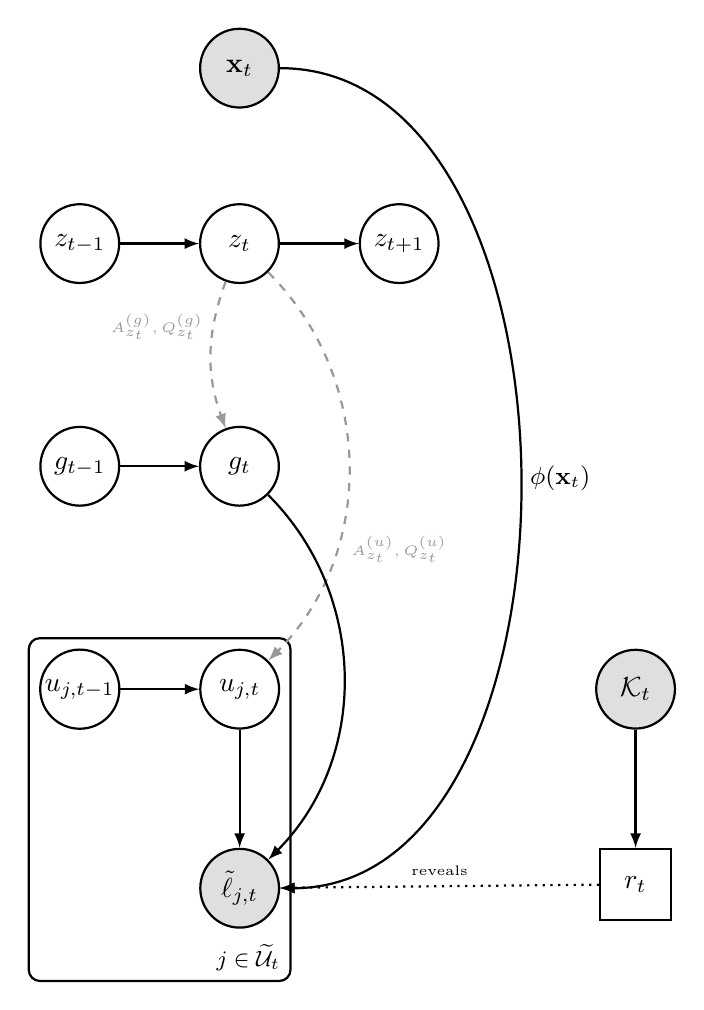
\begin{tikzpicture}[
    node distance=1.5cm and 3cm,
    >=latex,
    thick,
    latent_node/.style={latent, minimum size=1cm},
    obs_node/.style={obs, minimum size=1cm},
    action_node/.style={draw, rectangle, minimum size=0.9cm},
    param_edge/.style={->, dashed, color=gray!80}
]

% --- NODES ---
\node[latent_node] (zt_prev) {$z_{t-1}$};
\node[latent_node, right=of zt_prev] (zt) {$z_t$};
\node[latent_node, right=of zt] (zt_next) {$z_{t+1}$};

\node[obs_node, above=1.2cm of zt] (xt) {$\mathbf{x}_t$};

\node[latent_node, below=1.8cm of zt_prev] (gt_prev) {$g_{t-1}$};
\node[latent_node, right=of gt_prev] (gt) {$g_t$};

\node[latent_node, below=1.8cm of gt_prev] (ut_prev) {$u_{j,t-1}$};
\node[latent_node, right=of ut_prev] (ut) {$u_{j,t}$};

\node[obs_node, below=1.5cm of ut] (lt) {$\tilde{\ell}_{j,t}$};

% Plate over maintained registry (working set)
\plate {experts} {(ut_prev)(ut)(lt)} {$j \in \widetilde{\mathcal U}_t$};

% Availability and action
\node[obs_node, right=4cm of ut] (Kt) {$\Expert_t$};
\node[action_node, below=1.5cm of Kt] (rt) {$r_t$};

% --- EDGES ---
\edge {zt_prev} {zt};
\edge {zt} {zt_next};
\edge {gt_prev} {gt};
\edge {ut_prev} {ut};

\draw[param_edge] (zt) to [bend right=20] node[pos=0.3, left, font=\tiny] {$A^{(g)}_{z_t},Q^{(g)}_{z_t}$} (gt);
\draw[param_edge] (zt.south east) to [bend left=45] node[pos=0.7, right, font=\tiny, xshift=2pt] {$A^{(u)}_{z_t},Q^{(u)}_{z_t}$} (ut.north east);

\draw[->] (gt) to [bend left=45] (lt);
\edge {ut} {lt};

\draw[->] (xt.east) to [out=0, in=0, looseness=1] node[midway, right, font=\small] {$\phi(\mathbf{x}_t)$} (lt.east);

\edge {Kt} {rt};

% Selection affects what is observed (not what is generated)
\draw[->, dotted] (rt) -- (lt) node[midway, above, font=\tiny] {reveals};

\end{tikzpicture}
    \caption{Graphical model of the SLDS with partial feedback. The plate $j\in\widetilde{\mathcal U}_t$ denotes experts whose
    latent states are maintained by the filter; $\Expert_t$ restricts the action $r_t\in\Expert_t$. The action affects which loss is
    \emph{revealed} (censoring), not the underlying generative process.}
    \label{fig:slds_pgm_final}
\end{figure}


\section{Inference: Interacting Multiple Model (IMM) Filter}
\label{sec:imm}

Exact Bayesian filtering in an SLDS is intractable in general: the exact filtering distribution is a mixture over all
regime histories $(z_1,\dots,z_t)$, whose number grows as $M^t$ for $M$ regimes. We therefore use the
\emph{Interacting Multiple Model} (IMM) approximation, maintaining at each time $t$ a bank of $M$ regime-conditional
Gaussian filters and performing an \emph{interaction} (moment-matching) step at each transition.

\paragraph{Star-Gaussian approximation for scalable cross-expert dependence.}
The generative model couples experts through a shared factor $g_t$. Maintaining the full covariance of the stacked state
$\chi_t=(g_t,(u_{j,t})_{j})$ scales poorly with the number of experts.
We therefore adopt a \emph{star} Gaussian representation under each regime $k$:
we track the marginal moments of $g_t$ and each $u_{j,t}$, and the cross-covariances
\[
    \rho^{(k)}_{j,t\mid \cdot}\;\coloneqq\;\Cov\!\bigl(g_t,u_{j,t}\mid z_t=k,\cdot\bigr),
\]
but we do \emph{not} explicitly store $\Cov(u_{i,t},u_{j,t}\mid\cdot)$ for $i\neq j$.
This retains the main information-transfer mechanism (through $g_t$) while keeping inference linear in the number of experts.

\paragraph{Post-feedback history.}
Filtering is performed at the end of each round, after observing the selected loss. Define the post-feedback history
\[
    \mathcal I_t \;\coloneqq\; \bigl((\mathbf x_\tau,\Expert_\tau,G_\tau)\bigr)_{1\le \tau \le t},
    \qquad
    G_\tau \coloneqq (r_\tau,\tilde\ell_{r_\tau,\tau}),
\]
where $\tilde\ell_{r,t}\coloneqq \psi(\ell_{r,t})$ is the transformed loss (with $\psi=\mathrm{id}$ if no transform is used).
At decision time $t+1$, the router additionally observes $(\mathbf x_{t+1},\Expert_{t+1})$, i.e.
$H_{t+1}=(\mathcal I_t,\mathbf x_{t+1},\Expert_{t+1})$.

\subsection{Belief Representation (IMM + Star Gaussian)}

Let $\widetilde{\mathcal U}_t$ denote the working set of experts whose latent states are maintained by the filter
(after any pruning), and assume $\Expert_t\subseteq \widetilde{\mathcal U}_t$.
At the end of round $t$, the filter represents the posterior over $(z_t,g_t,(u_{j,t})_{j\in\widetilde{\mathcal U}_t})$ by:

\begin{enumerate}
    \item \textbf{Regime probabilities:}
    \[
        b_t(k) \;\coloneqq\; \mathbb P(z_t=k \mid \mathcal I_t),
        \qquad k\in\mathcal Z.
    \]

    \item \textbf{Regime-conditional star moments:} for each $k\in\mathcal Z$,
    \[
        g_t \mid \{z_t=k,\mathcal I_t\} \approx \Normal\!\bigl(m^{(k)}_{g,t\mid t},P^{(k)}_{g,t\mid t}\bigr),
        \qquad
        u_{j,t} \mid \{z_t=k,\mathcal I_t\} \approx \Normal\!\bigl(m^{(k)}_{u_j,t\mid t},P^{(k)}_{u_j,t\mid t}\bigr),
    \]
    and the cross-covariance blocks
    \[
        \rho^{(k)}_{j,t\mid t}\;\coloneqq\;\Cov\!\bigl(g_t,u_{j,t} \mid z_t=k,\mathcal I_t\bigr)
        \in\mathbb R^{d_g\times d_\alpha},
        \qquad j\in\widetilde{\mathcal U}_t.
    \]
\end{enumerate}

\subsection{Step 1: Interaction (Mixing Across Regimes)}

Define the predicted (one-step) regime prior
\[
    \bar b_{t+1\mid t}(k)\;\coloneqq\;\mathbb P(z_{t+1}=k\mid \mathcal I_t)
    \;=\;
    \sum_{i=1}^M b_t(i)\Pi_{ik}.
\]
For each candidate next regime $k$, define the IMM mixing weights
\[
    \mu_{i\mid k}
    \;\coloneqq\;
    \mathbb P(z_t=i\mid z_{t+1}=k,\mathcal I_t)
    \;=\;
    \frac{\Pi_{ik}b_t(i)}{\bar b_{t+1\mid t}(k)}.
\]

\paragraph{Moment matching in star form.}
For each candidate next regime $k$, we compute mixed moments at time $t$ (before time update).
For the shared factor:
\begin{align*}
    m^{0,(k)}_{g,t\mid t}
    &\;\coloneqq\;\sum_{i=1}^M \mu_{i\mid k}\,m^{(i)}_{g,t\mid t},\\
    P^{0,(k)}_{g,t\mid t}
    &\;\coloneqq\;\sum_{i=1}^M \mu_{i\mid k}
    \Bigl[P^{(i)}_{g,t\mid t}+\bigl(m^{(i)}_{g,t\mid t}-m^{0,(k)}_{g,t\mid t}\bigr)\bigl(m^{(i)}_{g,t\mid t}-m^{0,(k)}_{g,t\mid t}\bigr)^\top\Bigr].
\end{align*}
For each expert $j\in\widetilde{\mathcal U}_t$:
\begin{align*}
    m^{0,(k)}_{u_j,t\mid t}
    &\;\coloneqq\;\sum_{i=1}^M \mu_{i\mid k}\,m^{(i)}_{u_j,t\mid t},\\
    P^{0,(k)}_{u_j,t\mid t}
    &\;\coloneqq\;\sum_{i=1}^M \mu_{i\mid k}
    \Bigl[P^{(i)}_{u_j,t\mid t}+\bigl(m^{(i)}_{u_j,t\mid t}-m^{0,(k)}_{u_j,t\mid t}\bigr)\bigl(m^{(i)}_{u_j,t\mid t}-m^{0,(k)}_{u_j,t\mid t}\bigr)^\top\Bigr],\\
    \rho^{0,(k)}_{j,t\mid t}
    &\;\coloneqq\;\sum_{i=1}^M \mu_{i\mid k}
    \Bigl[\rho^{(i)}_{j,t\mid t}+\bigl(m^{(i)}_{g,t\mid t}-m^{0,(k)}_{g,t\mid t}\bigr)\bigl(m^{(i)}_{u_j,t\mid t}-m^{0,(k)}_{u_j,t\mid t}\bigr)^\top\Bigr].
\end{align*}

\subsection{Step 2: Time Update (Prediction) and Expert Birth}

Given candidate next regime $k$, propagate mixed moments from $t$ to $t+1$ using the regime-$k$ linear dynamics.
For the shared factor:
\begin{align}
    m^{(k)}_{g,t+1\mid t}
    &= A_k^{(g)}\, m^{0,(k)}_{g,t\mid t},\\
    P^{(k)}_{g,t+1\mid t}
    &= A_k^{(g)}\, P^{0,(k)}_{g,t\mid t}\,A_k^{(g)\top} + Q_k^{(g)}.
\end{align}
For each expert $j\in\widetilde{\mathcal U}_t$:
\begin{align}
    m^{(k)}_{u_j,t+1\mid t}
    &= A_k^{(u)}\, m^{0,(k)}_{u_j,t\mid t},\\
    P^{(k)}_{u_j,t+1\mid t}
    &= A_k^{(u)}\, P^{0,(k)}_{u_j,t\mid t}\,A_k^{(u)\top} + Q_k^{(u)},\\
    \rho^{(k)}_{j,t+1\mid t}
    &= A_k^{(g)}\, \rho^{0,(k)}_{j,t\mid t}\,A_k^{(u)\top},
\end{align}
using independence of process noises across $g$ and $u_j$.

\paragraph{Birth at time $t+1$.}
Let $\mathcal B_{t+1}\coloneqq \Expert_{t+1}\setminus \widetilde{\mathcal U}_t$ be the set of newly appearing experts
(at decision time $t+1$) not yet tracked. For each $j\in\mathcal B_{t+1}$ we append to the \emph{predicted} moments:
\begin{equation}
    \label{eq:imm_birth_append}
    m^{(k)}_{u_j,t+1\mid t} \;=\; m^{(k)}_{u,\mathrm{birth}},
    \qquad
    P^{(k)}_{u_j,t+1\mid t} \;=\; P^{(k)}_{u,\mathrm{birth}},
    \qquad
    \rho^{(k)}_{j,t+1\mid t}\;=\;0.
\end{equation}
We then set the working set to include the new experts:
$\widetilde{\mathcal U}_{t+1}\leftarrow \widetilde{\mathcal U}_t\cup \mathcal B_{t+1}$ (before any pruning).

\subsection{Step 3: Measurement Update (Partial Feedback)}

At round $t+1$ the router selects $r_{t+1}\in\Expert_{t+1}$ and observes the transformed loss $\tilde\ell_{r_{t+1},t+1}$.
Fix a regime $k\in\mathcal Z$ and write $r\coloneqq r_{t+1}$.
Under the emission model (Section~\ref{sec:observation-partial}),
\[
    \tilde\ell_{r,t+1}
    \;=\;
    \phi_{t+1}^\top(B_r g_{t+1}+u_{r,t+1}) + v_{r,t+1},
    \qquad v_{r,t+1}\sim \Normal(0,R_{k,r}).
\]
Define $a_{r,t+1}\coloneqq B_r^\top\phi_{t+1}\in\mathbb R^{d_g}$.
Then the regime-$k$ predicted mean and variance are
\begin{align}
    \hat{\tilde\ell}_{t+1}^{(k)}
    &\;\coloneqq\;
    \phi_{t+1}^\top\!\bigl(B_r m^{(k)}_{g,t+1\mid t}+m^{(k)}_{u_r,t+1\mid t}\bigr),\\
    S_{t+1}^{(k)}
    &\;\coloneqq\;
    a_{r,t+1}^\top P^{(k)}_{g,t+1\mid t} a_{r,t+1}
    +
    \phi_{t+1}^\top P^{(k)}_{u_r,t+1\mid t}\phi_{t+1}
    +
    2\,a_{r,t+1}^\top \rho^{(k)}_{r,t+1\mid t}\,\phi_{t+1}
    + R_{k,r},
\end{align}
and the innovation is
\[
    e_{t+1}^{(k)} \;\coloneqq\; \tilde\ell_{r,t+1} - \hat{\tilde\ell}_{t+1}^{(k)}.
\]

\paragraph{Regime-conditional gains and update for $(g_{t+1},u_{r,t+1})$.}
Define the gains
\begin{align}
    K^{(k)}_{g,t+1}
    &\;\coloneqq\;
    \frac{P^{(k)}_{g,t+1\mid t} a_{r,t+1} + \rho^{(k)}_{r,t+1\mid t} \phi_{t+1}}{S_{t+1}^{(k)}}
    \in\mathbb R^{d_g},\\
    K^{(k)}_{u_r,t+1}
    &\;\coloneqq\;
    \frac{\rho^{(k)\top}_{r,t+1\mid t} a_{r,t+1} + P^{(k)}_{u_r,t+1\mid t}\phi_{t+1}}{S_{t+1}^{(k)}}
    \in\mathbb R^{d_\alpha}.
\end{align}
Update means:
\begin{align}
    m^{(k)}_{g,t+1\mid t+1}
    &= m^{(k)}_{g,t+1\mid t} + K^{(k)}_{g,t+1}\, e_{t+1}^{(k)},\\
    m^{(k)}_{u_r,t+1\mid t+1}
    &= m^{(k)}_{u_r,t+1\mid t} + K^{(k)}_{u_r,t+1}\, e_{t+1}^{(k)}.
\end{align}
Update covariances and cross-covariance:
\begin{align}
    P^{(k)}_{g,t+1\mid t+1}
    &= P^{(k)}_{g,t+1\mid t} - K^{(k)}_{g,t+1}\, S_{t+1}^{(k)}\, K^{(k)\top}_{g,t+1},\\
    P^{(k)}_{u_r,t+1\mid t+1}
    &= P^{(k)}_{u_r,t+1\mid t} - K^{(k)}_{u_r,t+1}\, S_{t+1}^{(k)}\, K^{(k)\top}_{u_r,t+1},\\
    \rho^{(k)}_{r,t+1\mid t+1}
    &= \rho^{(k)}_{r,t+1\mid t} - K^{(k)}_{g,t+1}\, S_{t+1}^{(k)}\, K^{(k)\top}_{u_r,t+1}.
\end{align}

\paragraph{Unselected experts (indirect update through $g_{t+1}$).}
For each $j\neq r$ in $\widetilde{\mathcal U}_{t+1}$, there is no direct observation of $\tilde\ell_{j,t+1}$.
Under the star approximation, we propagate information gained about $g_{t+1}$ to $u_{j,t+1}$ by keeping the prior
conditional law $u_{j,t+1}\mid g_{t+1}$ fixed and updating only the marginal of $g_{t+1}$. This yields:
\begin{align}
    m^{(k)}_{u_j,t+1\mid t+1}
    &=
    m^{(k)}_{u_j,t+1\mid t}
    +
    \rho^{(k)\top}_{j,t+1\mid t}\,
    \bigl(P^{(k)}_{g,t+1\mid t}\bigr)^{-1}
    \bigl(m^{(k)}_{g,t+1\mid t+1}-m^{(k)}_{g,t+1\mid t}\bigr),\label{eq:star_unselected_mean}\\
    P^{(k)}_{u_j,t+1\mid t+1}
    &=
    P^{(k)}_{u_j,t+1\mid t}
    +
    \rho^{(k)\top}_{j,t+1\mid t}\,
    \bigl(P^{(k)}_{g,t+1\mid t}\bigr)^{-1}
    \bigl(P^{(k)}_{g,t+1\mid t+1}-P^{(k)}_{g,t+1\mid t}\bigr)
    \bigl(P^{(k)}_{g,t+1\mid t}\bigr)^{-1}
    \rho^{(k)}_{j,t+1\mid t},\label{eq:star_unselected_cov}\\
    \rho^{(k)}_{j,t+1\mid t+1}
    &=
    P^{(k)}_{g,t+1\mid t+1}\,
    \bigl(P^{(k)}_{g,t+1\mid t}\bigr)^{-1}\,
    \rho^{(k)}_{j,t+1\mid t}.\label{eq:star_unselected_rho}
\end{align}
Equations \eqref{eq:star_unselected_mean}--\eqref{eq:star_unselected_rho} are exact for Gaussians under the constraint that
$u_{j,t+1}\mid g_{t+1}$ is unchanged by the measurement; they implement the intended ``information propagation via $g$''.

\subsection{Step 4: Regime Probability Update}

Finally, update regime probabilities using the likelihood of the observed loss under each regime hypothesis. For each
$k\in\mathcal Z$, define the Gaussian likelihood
\[
    \Lambda_{t+1}^{(k)}
    \;\coloneqq\;
    \Normal\!\bigl(
        \tilde\ell_{r,t+1};
        \hat{\tilde\ell}_{t+1}^{(k)},
        S_{t+1}^{(k)}
    \bigr),
\]
and apply Bayes' rule with the predicted regime prior $\bar b_{t+1\mid t}(k)$:
\[
    b_{t+1}(k)
    \;\coloneqq\;
    \mathbb P(z_{t+1}=k \mid \mathcal I_{t+1})
    \;=\;
    \frac{\Lambda_{t+1}^{(k)} \, \bar b_{t+1\mid t}(k)}{\sum_{l=1}^M \Lambda_{t+1}^{(l)} \, \bar b_{t+1\mid t}(l)},
    \qquad k\in\mathcal Z.
\]

\begin{remark}[What is approximated]
IMM approximates the exact SLDS filter in two ways:
\begin{enumerate}[label=(\roman*)]
    \item \textbf{History truncation:} the exact filtering distribution is a mixture over regime histories
    $(z_1,\dots,z_t)$; IMM retains only the $M$ components indexed by $z_t$.
    \item \textbf{Moment matching / interaction:} for each candidate next regime $k$, the mixed prior over $z_t$ is a mixture
    of Gaussians; IMM replaces it by a single Gaussian matching first and second moments.
\end{enumerate}
In addition, the star representation is an \emph{extra approximation} that preserves the dependence structure mediated by
$g_t$ (via $\rho_{j,t}$) while discarding explicit $u_i$--$u_j$ covariance blocks.
\end{remark}

\section{Selection Policy}
\label{sec:policy}

At decision time $t+1$, the router observes
\[
    H_{t+1} \;=\; (\mathcal I_t,\mathbf x_{t+1},\Expert_{t+1}),
\]
i.e., the post-feedback history up to $t$, the current context $\mathbf x_{t+1}$ (hence $\phi_{t+1}$), and the currently
available expert set $\Expert_{t+1}$. Based on $H_{t+1}$, the router must choose an index
\(
    r_{t+1}\in\Expert_{t+1}.
\)

\paragraph{Cost.}
If expert $j$ were selected at time $t+1$, the one-step total cost is
\[
    C_{j,t+1} \;\coloneqq\; \ell_{j,t+1} + \beta_j,
\]
where $\beta_j\ge 0$ is deterministic and known at decision time.

\paragraph{Observation scale.}
The filter operates on the scalar observation
\[
    y_{j,t}\;\coloneqq\;\psi(\ell_{j,t}),
\]
where $\psi=\mathrm{id}$ by default (no transform). The linear-Gaussian emission in Section~\ref{sec:observation-partial}
is written for $y_{j,t}$. When $\psi\neq \mathrm{id}$, the policy below ranks experts using forecasts for $y_{j,t+1}$
(which is valid if $y$ is the operational loss proxy). If one wishes to optimize $\mathbb E[\ell_{j,t+1}\mid H_{t+1}]$
instead, one must push the predictive law of $y_{j,t+1}$ through $\psi^{-1}$ (log-normal closed form for
$\psi(x)=\log(x+\varepsilon)$; otherwise delta method / Monte Carlo).

\subsection{One-step Forecast under IMM + Star}

Because $\Pi$ is time-homogeneous and does not depend on $\mathbf x$, the predicted regime probabilities at decision time
$t+1$ are
\[
    \bar b_{t+1\mid t}(k)
    \;\coloneqq\;
    \mathbb P(z_{t+1}=k\mid \mathcal I_t)
    \;=\;
    \sum_{i=1}^M b_t(i)\Pi_{ik},
    \qquad k\in\mathcal Z.
\]
For each $k\in\mathcal Z$, the IMM time-update provides the star predictive moments
\[
    (m^{(k)}_{g,t+1\mid t},P^{(k)}_{g,t+1\mid t}),\quad
    (m^{(k)}_{u_j,t+1\mid t},P^{(k)}_{u_j,t+1\mid t}),\quad
    \rho^{(k)}_{j,t+1\mid t}=\Cov(g_{t+1},u_{j,t+1}\mid z_{t+1}=k,\mathcal I_t)
\]
for all experts $j$ in the maintained registry (after any birth step).

Fix $j$ and define
\[
    a_{j,t+1}\;\coloneqq\;B_j^\top\phi_{t+1}\in\mathbb R^{d_g}.
\]
Under regime $z_{t+1}=k$, the star predictor yields the Gaussian forecast
\[
    y_{j,t+1}\mid\{z_{t+1}=k,H_{t+1}\}
    \;\approx\;
    \Normal\!\bigl(\mu^{(k)}_{j,t+1\mid t},\,\sigma^{2,(k)}_{j,t+1\mid t}\bigr),
\]
with mean
\begin{equation}
\label{eq:sel_mu_star}
    \mu^{(k)}_{j,t+1\mid t}
    \;\coloneqq\;
    a_{j,t+1}^\top m^{(k)}_{g,t+1\mid t} + \phi_{t+1}^\top m^{(k)}_{u_j,t+1\mid t},
\end{equation}
and variance
\begin{equation}
\label{eq:sel_var_star}
    \sigma^{2,(k)}_{j,t+1\mid t}
    \;\coloneqq\;
    a_{j,t+1}^\top P^{(k)}_{g,t+1\mid t} a_{j,t+1}
    + \phi_{t+1}^\top P^{(k)}_{u_j,t+1\mid t} \phi_{t+1}
    + 2\,a_{j,t+1}^\top \rho^{(k)}_{j,t+1\mid t}\,\phi_{t+1}
    + R_{k,j}.
\end{equation}

Therefore, the IMM predictive law is the mixture
\[
    \mathbb P(y_{j,t+1}\mid H_{t+1})
    \;\approx\;
    \sum_{k=1}^M \bar b_{t+1\mid t}(k)\,
    \Normal\!\bigl(\cdot;\mu^{(k)}_{j,t+1\mid t},\,\sigma^{2,(k)}_{j,t+1\mid t}\bigr).
\]

\paragraph{Predictive mean.}
The one-step point forecast (squared-loss optimal on the $y$-scale) is
\begin{equation}
\label{eq:sel_mean_mix_star}
    \widehat y_{j,t+1\mid t}
    \;\coloneqq\;
    \mathbb E[y_{j,t+1}\mid H_{t+1}]
    \;\approx\;
    \sum_{k=1}^M \bar b_{t+1\mid t}(k)\,\mu^{(k)}_{j,t+1\mid t}.
\end{equation}

\subsection{Predictive Variance (State + Regime Uncertainty)}

Define the conditional predictive variance on the observation scale
\[
    \widehat\sigma^2_{j,t+1\mid t}\;\coloneqq\;\Var(y_{j,t+1}\mid H_{t+1}).
\]

\begin{proposition}[Total variance under IMM]\label{prop:total_variance_star}
For each expert $j$,
\begin{equation}
\label{eq:total_variance_star}
    \widehat\sigma^2_{j,t+1\mid t}
    \;\approx\;
    \sum_{k=1}^M \bar b_{t+1\mid t}(k)\,\sigma^{2,(k)}_{j,t+1\mid t}
    \;+\;
    \sum_{k=1}^M \bar b_{t+1\mid t}(k)\,
    \bigl(\mu^{(k)}_{j,t+1\mid t}-\widehat y_{j,t+1\mid t}\bigr)^2,
\end{equation}
where $\widehat y_{j,t+1\mid t}$ is defined in \eqref{eq:sel_mean_mix_star}.
\end{proposition}

\begin{proof}
Apply the law of total variance with $Y=y_{j,t+1}$ and $Z=z_{t+1}$, conditioning on $H_{t+1}$:
\[
    \Var(Y\mid H_{t+1})
    =
    \mathbb E[\Var(Y\mid Z,H_{t+1})\mid H_{t+1}]
    +
    \Var(\mathbb E[Y\mid Z,H_{t+1}]\mid H_{t+1}),
\]
and plug in the IMM weights $\bar b_{t+1\mid t}(k)$ and the regime-conditional moments
$\mu^{(k)}_{j,t+1\mid t}$, $\sigma^{2,(k)}_{j,t+1\mid t}$.
\end{proof}

\subsection{Cost-sensitive Risk-adjusted Rule}

For each available expert $j\in\Expert_{t+1}$, define the risk-adjusted score (on the filter scale)
\[
    J_{j,t+1}
    \;\coloneqq\;
    \widehat y_{j,t+1\mid t}
    + \beta_j
    + \lambda \sqrt{\widehat\sigma^2_{j,t+1\mid t}},
\]
where $\lambda\in\mathbb R$ is a user-specified risk parameter. The router selects
\begin{equation}
    \label{eq:policy_star}
    r_{t+1}^\star \in \arg\min_{j\in\Expert_{t+1}} J_{j,t+1}.
\end{equation}
For $\lambda=0$, this is the myopic mean-cost rule (on the $y$-scale). For $\lambda>0$, the policy penalizes predictive
uncertainty.

\begin{proposition}[Tail control via Cantelli (conditional)]
\label{prop:cantelli_star}
Fix $t$ and condition on $H_{t+1}$. For any expert $j\in\Expert_{t+1}$, let
\[
    m_j \coloneqq \mathbb E[y_{j,t+1}+\beta_j\mid H_{t+1}],
    \qquad
    s_j^2 \coloneqq \Var(y_{j,t+1}+\beta_j\mid H_{t+1})=\Var(y_{j,t+1}\mid H_{t+1}).
\]
Then for any $\lambda>0$,
\[
    \mathbb P\!\left(
        y_{j,t+1}+\beta_j - m_j \ge \lambda s_j \,\middle|\, H_{t+1}
    \right)
    \;\le\;
    \frac{1}{1+\lambda^2}.
\]
\end{proposition}

\begin{proof}
Cantelli's inequality applied conditionally on $H_{t+1}$.
\end{proof}

\paragraph{Regime-dependent risk aversion.}
If risk tolerance differs across regimes, specify $\bm\lambda=(\lambda^{(1)},\dots,\lambda^{(M)})$ and use the
decision-time effective risk parameter
\[
    \bar\lambda_{t+1\mid t}\;\coloneqq\;\sum_{k=1}^M \bar b_{t+1\mid t}(k)\,\lambda^{(k)}.
\]
Replace $\lambda$ by $\bar\lambda_{t+1\mid t}$ in $J_{j,t+1}$.

\section{Parameter Optimization}
\label{sec:param-opt}

We treat the feature map $\phi:\mathcal X\to\mathbb R^{d_\alpha}$ and the loadings $(B_j)$ as fixed, and learn the
remaining SLDS parameters:
\[
    \Theta
    \;\coloneqq\;
    \Bigl(
        \Pi,\ \mu^0,\ (A^{(g)}_k,Q^{(g)}_k)_{k=1}^M,\ (A^{(u)}_k,Q^{(u)}_k)_{k=1}^M,\
        (R_{k,j})_{\substack{k=1,\dots,M\\ j\in\mathcal U_T}}
    \Bigr).
\]
Here $\Pi\in[0,1]^{M\times M}$ is the regime transition matrix (independent of $\mathbf x$), $\mu^0$ the initial regime
distribution, and the remaining parameters are defined in
\eqref{eq:global_factor_transition}--\eqref{eq:idiosyncratic_transition} and \eqref{eq:observation_factor}.

\paragraph{Observed data (bandit feedback).}
We observe one scalar per round:
\[
    \mathbf D
    \;\coloneqq\;
    \{(\mathbf x_t,\Expert_t,r_t,y_{r_t,t})\}_{t=1}^T,
    \qquad
    y_{r_t,t}=\psi(\ell_{r_t,t}).
\]

\subsection{Controlled (Conditional) Maximum Likelihood}

Under the exogeneity assumption, the router's choice affects only \emph{which component is revealed}.
Accordingly we maximize the marginal likelihood of the observed sequence of revealed observations, \emph{conditioning on}
the realized censoring/selection pattern $(\Expert_t,r_t)_{t=1}^T$:
\begin{equation}
\label{eq:cond_mle}
    \mathcal J(\Theta)
    \;\coloneqq\;
    \sum_{t=1}^T
    \log p_\Theta\!\left(y_{r_t,t}\mid H_t, r_t\right),
    \qquad
    H_t=(\mathcal I_{t-1},\mathbf x_t,\Expert_t).
\end{equation}

\paragraph{IMM predictive mixture used in practice.}
Exact SLDS prediction is intractable for $M\ge2$. Using IMM+star, we approximate the one-step predictive density by
\begin{equation}
\label{eq:imm_pred_density}
    \tilde p_\Theta^{\mathrm{IMM}}(y_{r_t,t}\mid H_t,r_t)
    \;\coloneqq\;
    \sum_{k=1}^M \bar b_{t\mid t-1}(k)\,\Lambda_t^{(k)},
\end{equation}
where $\bar b_{t\mid t-1}(k)=\mathbb P_\Theta(z_t=k\mid \mathcal I_{t-1})$ is the IMM predictor and $\Lambda_t^{(k)}$ is
the regime-$k$ Gaussian likelihood under the star predictor.

Let $\phi_t=\phi(\mathbf x_t)$ and $r=r_t$. Define $a_{r,t}\coloneqq B_r^\top\phi_t\in\mathbb R^{d_g}$.
Under regime $k$, the star predictor provides
\(
(m^{(k)}_{g,t\mid t-1},P^{(k)}_{g,t\mid t-1}),
(m^{(k)}_{u_r,t\mid t-1},P^{(k)}_{u_r,t\mid t-1}),
\rho^{(k)}_{r,t\mid t-1}
\).
Then
\[
    \Lambda_t^{(k)}
    =
    \Normal\!\bigl(
        y_{r,t};
        \mu^{(k)}_{r,t\mid t-1},
        \sigma^{2,(k)}_{r,t\mid t-1}
    \bigr),
\]
with
\begin{align}
\label{eq:ll_mu_star2}
    \mu^{(k)}_{r,t\mid t-1}
    &\;\coloneqq\;
    a_{r,t}^\top m^{(k)}_{g,t\mid t-1} + \phi_t^\top m^{(k)}_{u_r,t\mid t-1},
    \\
\label{eq:ll_var_star2}
    \sigma^{2,(k)}_{r,t\mid t-1}
    &\;\coloneqq\;
    a_{r,t}^\top P^{(k)}_{g,t\mid t-1} a_{r,t}
    + \phi_t^\top P^{(k)}_{u_r,t\mid t-1}\phi_t
    + 2\,a_{r,t}^\top \rho^{(k)}_{r,t\mid t-1}\phi_t
    + R_{k,r}.
\end{align}
We therefore optimize the surrogate log-likelihood
\begin{equation}
\label{eq:imm_surrogate_ll}
    \tilde{\mathcal J}_{\mathrm{IMM}}(\Theta)
    \;\coloneqq\;
    \sum_{t=1}^T
    \log \tilde p_\Theta^{\mathrm{IMM}}(y_{r_t,t}\mid H_t,r_t).
\end{equation}

\subsection{Generalized EM with IMM + Star Smoothing}

We use generalized EM: an IMM forward pass and an approximate backward smoother yield an approximate posterior
$q^{(m)}$ under $\Theta^{(m)}$, and the M-step increases
\[
    Q(\Theta;\Theta^{(m)})
    \;\coloneqq\;
    \mathbb E_{q^{(m)}}\!\left[\log p_\Theta(\mathbf D,Z_{1:T},G_{1:T},U_{1:T})\right].
\]

\paragraph{E-step outputs.}
The smoother provides approximate regime marginals and pairwise marginals:
\[
    \gamma_t^{(k)} \approx \mathbb P(z_t=k\mid \mathcal I_T),
    \qquad
    \xi_t^{(i,k)} \approx \mathbb P(z_{t-1}=i,z_t=k\mid \mathcal I_T),
\]
and regime-conditional star-Gaussian moments (for all experts defined at time $t$):
\[
    (g_t,u_{j,t})\mid\{z_t=k,\mathcal I_T\}
    \approx
    \Normal\!\left(
        \begin{bmatrix} m^{(k)}_{g,t\mid T}\\ m^{(k)}_{u_j,t\mid T}\end{bmatrix},
        \begin{bmatrix}
            P^{(k)}_{g,t\mid T} & \rho^{(k)}_{j,t\mid T}\\
            \rho^{(k)\top}_{j,t\mid T} & P^{(k)}_{u_j,t\mid T}
        \end{bmatrix}
    \right),
\]
together with lag-one covariances for the linear dynamics:
\[
    P^{(k)}_{g,t,t-1\mid T}\approx \Cov(g_t,g_{t-1}\mid z_t=k,\mathcal I_T),
    \qquad
    P^{(k)}_{u_j,t,t-1\mid T}\approx \Cov(u_{j,t},u_{j,t-1}\mid z_t=k,\mathcal I_T).
\]

\subsection{M-step (Closed-form Updates)}

\paragraph{Initial regime distribution.}
\[
    \mu^{0,(m+1)}_k \;=\; \gamma_1^{(k)}.
\]

\paragraph{Regime transitions.}
For $i,k\in\mathcal Z$,
\[
     \Pi_{ik}^{(m+1)}
     \;=\;
    \frac{\sum_{t=2}^T \xi_t^{(i,k)}}{\sum_{t=2}^T \sum_{k'=1}^M \xi_t^{(i,k')}}.
\]

\paragraph{Factor dynamics $(A^{(g)}_k,Q^{(g)}_k)$.}
Because the dynamics are indexed by $z_t$ (i.e.\ the regime at time $t$ governs the transition $t\!-\!1\to t$),
we weight by $\gamma_t^{(k)}$ for $t\ge2$. For each $k\in\mathcal Z$, define
\begin{align*}
    S^{(k)}_{11,g} &\coloneqq \sum_{t=2}^T \gamma_t^{(k)}\,
    \mathbb E[g_{t-1}g_{t-1}^\top \mid z_t=k,\mathcal I_T],\\
    S^{(k)}_{10,g} &\coloneqq \sum_{t=2}^T \gamma_t^{(k)}\,
    \mathbb E[g_{t}g_{t-1}^\top \mid z_t=k,\mathcal I_T],\\
    S^{(k)}_{00,g} &\coloneqq \sum_{t=2}^T \gamma_t^{(k)}\,
    \mathbb E[g_{t}g_{t}^\top \mid z_t=k,\mathcal I_T].
\end{align*}
Under the Gaussian approximation,
\[
    \mathbb E[g_t g_t^\top \mid z_t=k,\mathcal I_T]
    = P^{(k)}_{g,t\mid T} + m^{(k)}_{g,t\mid T} m^{(k)\top}_{g,t\mid T},
\quad
    \mathbb E[g_t g_{t-1}^\top \mid z_t=k,\mathcal I_T]
    = P^{(k)}_{g,t,t-1\mid T} + m^{(k)}_{g,t\mid T} m^{(k)\top}_{g,t-1\mid T}.
\]
If $S^{(k)}_{11,g}$ is invertible,
\[
    A^{(g),(m+1)}_k \;=\; S^{(k)}_{10,g}\bigl(S^{(k)}_{11,g}\bigr)^{-1},
\qquad
    Q^{(g),(m+1)}_k
    \;=\;
    \frac{1}{\sum_{t=2}^T \gamma_t^{(k)}}
    \Bigl(S^{(k)}_{00,g} - A^{(g),(m+1)}_k S^{(k)\top}_{10,g}\Bigr),
\]
followed by symmetrization/projection onto $\mathbb S_{+}^{d_g}$ if needed.

\paragraph{Idiosyncratic dynamics $(A^{(u)}_k,Q^{(u)}_k)$.}
Let $\tau_j$ be the birth time of expert $j$. For each $k\in\mathcal Z$, define
\begin{align*}
    S^{(k)}_{11,u} &\coloneqq \sum_{j\in\mathcal U_T}\sum_{t=\tau_j+1}^T \gamma_t^{(k)}\,
    \mathbb E[u_{j,t-1}u_{j,t-1}^\top \mid z_t=k,\mathcal I_T],\\
    S^{(k)}_{10,u} &\coloneqq \sum_{j\in\mathcal U_T}\sum_{t=\tau_j+1}^T \gamma_t^{(k)}\,
    \mathbb E[u_{j,t}u_{j,t-1}^\top \mid z_t=k,\mathcal I_T],\\
    S^{(k)}_{00,u} &\coloneqq \sum_{j\in\mathcal U_T}\sum_{t=\tau_j+1}^T \gamma_t^{(k)}\,
    \mathbb E[u_{j,t}u_{j,t}^\top \mid z_t=k,\mathcal I_T].
\end{align*}
If $S^{(k)}_{11,u}$ is invertible,
\[
    A^{(u),(m+1)}_k \;=\; S^{(k)}_{10,u}\bigl(S^{(k)}_{11,u}\bigr)^{-1},
\qquad
    Q^{(u),(m+1)}_k
    \;=\;
    \frac{1}{\sum_{j\in\mathcal U_T}\sum_{t=\tau_j+1}^T \gamma_t^{(k)}}
    \Bigl(S^{(k)}_{00,u} - A^{(u),(m+1)}_k S^{(k)\top}_{10,u}\Bigr),
\]
with symmetrization/projection if needed.

\paragraph{Observation noise $R_{k,j}$.}
Only times when expert $j$ is selected contribute. Let $\phi_t=\phi(\mathbf x_t)$ and $a_{j,t}=B_j^\top\phi_t$.
For each $(k,j)$ define
\[
    \hat y^{(k)}_{j,t}
    \;\coloneqq\;
    a_{j,t}^\top m^{(k)}_{g,t\mid T} + \phi_t^\top m^{(k)}_{u_j,t\mid T},
\]
and the explained variance under the star posterior
\[
    \hat v^{(k)}_{j,t}
    \;\coloneqq\;
    a_{j,t}^\top P^{(k)}_{g,t\mid T} a_{j,t}
    + \phi_t^\top P^{(k)}_{u_j,t\mid T} \phi_t
    + 2\,a_{j,t}^\top \rho^{(k)}_{j,t\mid T} \phi_t.
\]
Then the M-step update is
\[
    R_{k,j}^{(m+1)}
    \;=\;
    \frac{\sum_{t:\,r_t=j}\gamma_t^{(k)}\Bigl[(y_{j,t}-\hat y^{(k)}_{j,t})^2+\hat v^{(k)}_{j,t}\Bigr]}
         {\sum_{t:\,r_t=j}\gamma_t^{(k)}}.
\]
If the denominator is zero (expert $j$ never selected in regime $k$ under the smoother), one should keep $R_{k,j}$
unchanged, tie it across experts (e.g.\ $R_{k,j}\equiv R_k$), or use a prior/shrinkage update.

\begin{remark}[Identifiability under bandit feedback]
Because only the selected expert is observed, expert-specific observation variances $R_{k,j}$ (and any untied
expert-specific parameters) are weakly identified for rarely queried experts. In practice, one typically ties parameters
(e.g.\ $R_{k,j}\equiv R_k$ or $R_{k,j}\equiv R$), uses informative priors, and/or enforces exploration to avoid
degeneracy.
\end{remark}

\section{Extension: Full-Information Expert Feedback}
\label{sec:full-info}

In the main development, the router observes at each time $t$ only the loss of the selected expert $r_t$, yielding censored
(bandit-style) feedback. In some applications (e.g.\ all experts are models evaluated once the ground-truth is revealed),
it is natural to assume a \emph{full-information} setting: after each epoch, the losses of \emph{all available} experts can
be computed, regardless of which expert was queried for decision-making.

This section formalizes the full-information feedback model and the corresponding modifications to SLDS--IMM inference and
to routing.

\subsection{Feedback model with full expert losses}

We retain the generative model of Sections~\ref{sec:slds}--\ref{sec:imm} together with the shared-factor reliability model
(Option~A with star covariance tracking) from Section~\ref{sec:observation-partial}. Write
$\phi_t\coloneqq \phi(\mathbf x_t)\in\mathbb R^{d_\alpha}$. Conditionally on $z_t=k$, for every expert $j\in\mathcal U_t$
(the registry at time $t$), the loss is generated by the same linear-Gaussian emission:
\begin{equation}
\label{eq:fullinfo_emission}
    \ell_{j,t}
    \;=\;
    \phi_t^\top\!\bigl(B_j g_t + u_{j,t}\bigr)
    + v_{j,t},
    \qquad
    v_{j,t}\sim\mathcal N(0,R_{k,j}),
\end{equation}
with $(v_{j,t})_{j,t}$ independent across $j$ and $t$, and independent of the latent states conditional on
$(z_t,g_t,(u_{j,t})_{j\in\mathcal U_t})$. (If a monotone transform $\psi$ is used, \eqref{eq:fullinfo_emission} is understood
as applying to $\tilde\ell_{j,t}=\psi(\ell_{j,t})$.)

\paragraph{Decision-time information and full feedback.}
At time $t$, before observing any losses at $t$, the router observes
\[
    H_t^{\mathrm{full}}
    \;\coloneqq\;
    \bigl(\mathcal I_{t-1}^{\mathrm{full}},\,\mathbf x_t,\,\Expert_t\bigr),
\]
where the post-feedback history up to $t-1$ is
\[
    \mathcal I_{t-1}^{\mathrm{full}}
    \;\coloneqq\;
    \bigl( (\mathbf x_\tau,\Expert_\tau,G_\tau^{\mathrm{full}}) \bigr)_{1\le \tau \le t-1},
    \qquad
    \mathcal I_0^{\mathrm{full}} \text{ empty}.
\]
The router selects $r_t\in\Expert_t$. After the outcome is revealed, the system provides the \emph{full panel} of losses
for all available experts:
\[
    (\ell_{j,t})_{j\in\Expert_t}.
\]
We encode the post-decision feedback as
\[
    G_t^{\mathrm{full}}
    \;\coloneqq\;
    \bigl(r_t,\ (\ell_{j,t})_{j\in\Expert_t}\bigr),
\]
and set
\[
    \mathcal I_t^{\mathrm{full}}
    \;\coloneqq\;
    \bigl( (\mathbf x_\tau,\Expert_\tau,G_\tau^{\mathrm{full}}) \bigr)_{1\le \tau \le t}.
\]

\paragraph{Action-independence of the environment.}
As in the base model, we assume the latent/context process
\[
    \Bigl(z_t,\ g_t,\ (u_{j,t})_{j\in\mathcal U_t},\ \mathbf x_t\Bigr)_{t\ge 1}
\]
evolves independently of the routing decisions $(r_t)_{t\ge 1}$. The router affects only the incurred cost, not the
data-generating mechanism.

\subsection{IMM belief update under full feedback (IMM + star projection)}

Under full information, the filter can incorporate at each time $t$ the losses of \emph{all} $j\in\Expert_t$, rather than
only the selected expert. Steps 1--2 of IMM (interaction/mixing and time update) are unchanged.

Fix $t\ge 1$ and a regime $k\in\mathcal Z$. After interaction and time update, we have (star) predictive moments under $k$:
\[
    g_t \mid \{z_t=k,\mathcal I_{t-1}^{\mathrm{full}}\}
    \approx \mathcal N\!\bigl(m^{(k)}_{g,t\mid t-1},P^{(k)}_{g,t\mid t-1}\bigr),
\]
and for each $j\in\mathcal U_t$,
\[
    u_{j,t} \mid \{z_t=k,\mathcal I_{t-1}^{\mathrm{full}}\}
    \approx \mathcal N\!\bigl(m^{(k)}_{u_j,t\mid t-1},P^{(k)}_{u_j,t\mid t-1}\bigr),
    \qquad
    \rho^{(k)}_{j,t\mid t-1}\coloneqq \Cov(g_t,u_{j,t}\mid z_t=k,\mathcal I_{t-1}^{\mathrm{full}}).
\]
The star approximation sets $\Cov(u_{i,t},u_{j,t}\mid z_t=k,\mathcal I_{t-1}^{\mathrm{full}})\approx 0$ for $i\neq j$.

\paragraph{Panel observation model at time $t$.}
For each available expert $j\in\Expert_t$, define the scalar loading
\[
    a_{j,t} \;\coloneqq\; B_j^\top \phi_t\in\mathbb R^{d_g}.
\]
Then, conditional on $z_t=k$,
\[
    \ell_{j,t}
    \;=\;
    a_{j,t}^\top g_t + \phi_t^\top u_{j,t} + v_{j,t},
    \qquad v_{j,t}\sim\mathcal N(0,R_{k,j}).
\]

\paragraph{Batch update on the observed substate (exact under the star prior).}
Let $\Expert_t=\{j_1,\dots,j_m\}$ with $m\coloneqq|\Expert_t|$, and define the stacked substate
\[
    x_t^{(\Expert)} \;\coloneqq\; \bigl(g_t,\ u_{j_1,t},\dots,u_{j_m,t}\bigr).
\]
Under regime $k$, its predictive mean and covariance are
\[
    m^{(k)}_{x,t\mid t-1}
    \;=\;
    \begin{bmatrix}
        m^{(k)}_{g,t\mid t-1}\\
        m^{(k)}_{u_{j_1},t\mid t-1}\\
        \vdots\\
        m^{(k)}_{u_{j_m},t\mid t-1}
    \end{bmatrix},
    \qquad
    P^{(k)}_{x,t\mid t-1}
    \;=\;
    \begin{bmatrix}
        P^{(k)}_{g,t\mid t-1} & \rho^{(k)}_{j_1,t\mid t-1} & \cdots & \rho^{(k)}_{j_m,t\mid t-1}\\
        \rho^{(k)\top}_{j_1,t\mid t-1} & P^{(k)}_{u_{j_1},t\mid t-1} & \cdots & 0\\
        \vdots & \vdots & \ddots & \vdots\\
        \rho^{(k)\top}_{j_m,t\mid t-1} & 0 & \cdots & P^{(k)}_{u_{j_m},t\mid t-1}
    \end{bmatrix}.
\]
Define the panel observation vector $y_t\coloneqq (\ell_{j_s,t})_{s=1}^m\in\mathbb R^m$ and the observation matrix
$H_t\in\mathbb R^{m\times(d_g+m d_\alpha)}$ by, for each $s=1,\dots,m$,
\[
    (H_t)_{s,:}
    \;\coloneqq\;
    \bigl[a_{j_s,t}^\top\ \ \ 0\ \cdots\ 0\ \ \phi_t^\top\ \ 0\ \cdots\ 0\bigr],
\]
where $\phi_t^\top$ sits in the block corresponding to $u_{j_s,t}$. Let
\[
    R_t^{(k)} \;\coloneqq\; \mathrm{diag}(R_{k,j_1},\dots,R_{k,j_m}).
\]
Then the (regime-$k$) innovation covariance, gain, and batch update are
\[
    S_t^{(k)} \;\coloneqq\; H_t P^{(k)}_{x,t\mid t-1} H_t^\top + R_t^{(k)},
    \qquad
    K_t^{(k)} \;\coloneqq\; P^{(k)}_{x,t\mid t-1} H_t^\top (S_t^{(k)})^{-1},
\]
\begin{align}
\label{eq:fullinfo_batch_kf}
    m^{(k)}_{x,t\mid t}
    &= m^{(k)}_{x,t\mid t-1} + K_t^{(k)}\bigl(y_t - H_t m^{(k)}_{x,t\mid t-1}\bigr),\\
    P^{(k)}_{x,t\mid t}
    &= P^{(k)}_{x,t\mid t-1} - K_t^{(k)} S_t^{(k)} K_t^{(k)\top}. \nonumber
\end{align}

\paragraph{Star projection back to tracked moments.}
The exact posterior covariance $P^{(k)}_{x,t\mid t}$ generally contains nonzero cross-covariances between distinct
$u_{j_s,t}$ blocks. Under Option~A we \emph{project} back to the star family by retaining only:
\[
    (m^{(k)}_{g,t\mid t},P^{(k)}_{g,t\mid t}),
    \quad
    (m^{(k)}_{u_{j_s},t\mid t},P^{(k)}_{u_{j_s},t\mid t})\ (s=1,\dots,m),
    \quad
    \rho^{(k)}_{j_s,t\mid t}\ (s=1,\dots,m),
\]
as read off from the corresponding blocks of $m^{(k)}_{x,t\mid t}$ and $P^{(k)}_{x,t\mid t}$, and setting
$\Cov(u_{j_s,t},u_{j_{s'},t}\mid z_t=k,\mathcal I_t^{\mathrm{full}})\approx 0$ for $s\neq s'$.
Experts $j\notin\Expert_t$ are unobserved at time $t$; their star moments remain at the predictive values
$(m^{(k)}_{u_j,t\mid t},P^{(k)}_{u_j,t\mid t},\rho^{(k)}_{j,t\mid t})
\approx
(m^{(k)}_{u_j,t\mid t-1},P^{(k)}_{u_j,t\mid t-1},\rho^{(k)}_{j,t\mid t-1})$,
optionally followed by an ``indirect'' update driven by the updated $(m^{(k)}_{g,t\mid t},P^{(k)}_{g,t\mid t})$ (as in the
bandit case) if one wants to propagate information about $g_t$ to inactive experts.

\paragraph{Regime probability update (exact panel likelihood under the star prior).}
Under regime $k$, the panel predictive density is multivariate Gaussian:
\[
    y_t \ \big|\ \{z_t=k,\mathcal I_{t-1}^{\mathrm{full}},\mathbf x_t,\Expert_t\}
    \;\sim\;
    \mathcal N\!\bigl(H_t m^{(k)}_{x,t\mid t-1},\ S_t^{(k)}\bigr),
\]
so we set the regime likelihood
\[
    \Lambda_t^{(k)}
    \;\coloneqq\;
    \mathcal N\!\bigl(y_t;\ H_t m^{(k)}_{x,t\mid t-1},\ S_t^{(k)}\bigr).
\]
Let $b_{t-1}(i)\coloneqq \mathbb P(z_{t-1}=i\mid \mathcal I_{t-1}^{\mathrm{full}})$ and define the one-step regime predictor
\[
    \bar c_t(k)
    \;\coloneqq\;
    \mathbb P(z_t=k\mid \mathcal I_{t-1}^{\mathrm{full}})
    \;=\;
    \sum_{i=1}^M b_{t-1}(i)\,\Pi_{ik}.
\]
Bayes' rule yields
\[
    b_t(k)
    \;\coloneqq\;
    \mathbb P(z_t=k\mid \mathcal I_{t}^{\mathrm{full}})
    \;=\;
    \frac{\Lambda_t^{(k)}\,\bar c_t(k)}{\sum_{\ell=1}^M \Lambda_t^{(\ell)}\,\bar c_t(\ell)},
    \qquad k\in\mathcal Z.
\]
In implementation, compute $\log\Lambda_t^{(k)}$ via a Cholesky factorization of $S_t^{(k)}$ to avoid underflow.

\subsection{Consequences for the routing problem}

At decision time $t+1$, the router observes
\[
    H_{t+1}^{\mathrm{full}} = (\mathcal I_t^{\mathrm{full}},\mathbf x_{t+1},\Expert_{t+1})
\]
and selects $r_{t+1}\in\Expert_{t+1}$. Predictive means/variances for each expert are computed exactly as in the bandit case,
but conditioning on $\mathcal I_t^{\mathrm{full}}$.

Crucially, decisions no longer affect what is learned: at each time $t$ the full vector $(\ell_{j,t})_{j\in\Expert_t}$ is
observed regardless of which expert is chosen. Under action-independence, there is no exploration--exploitation coupling in
the expected-sum objective.

\begin{proposition}[Optimality of the myopic Bayes rule under full feedback]
\label{prop:myopic_opt_full}
Assume full-information feedback and action-independence of
$\bigl(z_t,g_t,(u_{j,t})_{j\in\mathcal U_t},\mathbf x_t\bigr)_{t=1}^T$ from $(r_t)_{t=1}^T$.
Define the one-step cost $C_t(j)\coloneqq \ell_{j,t}+\beta_j$. Then an optimal policy for
\[
    \inf_{\pi}\ \mathbb E\Bigl[\sum_{t=1}^T C_t(r_t)\Bigr]
\]
is obtained by choosing, at each time $t$,
\[
    r_t^\star
    \in
    \arg\min_{j\in\Expert_t}
    \mathbb E\!\left[C_t(j)\mid \mathcal I_{t-1}^{\mathrm{full}},\mathbf x_t,\Expert_t\right].
\]
\end{proposition}

\begin{proof}
By action-independence, conditional on the decision-time information $(\mathcal I_{t-1}^{\mathrm{full}},\mathbf x_t,\Expert_t)$,
the conditional law of $(C_t(j))_{j\in\Expert_t}$ does not depend on past or current actions. Using the tower property,
\[
    \mathbb E\Bigl[\sum_{t=1}^T C_t(r_t)\Bigr]
    =
    \sum_{t=1}^T
    \mathbb E\Bigl[
        \mathbb E\bigl[C_t(r_t)\mid \mathcal I_{t-1}^{\mathrm{full}},\mathbf x_t,\Expert_t\bigr]
    \Bigr].
\]
For each $t$, the inner conditional expectation is minimized by selecting
$r_t^\star\in\arg\min_{j\in\Expert_t}\mathbb E[C_t(j)\mid \mathcal I_{t-1}^{\mathrm{full}},\mathbf x_t,\Expert_t]$.
Since no action influences future conditional distributions, choosing $r_t^\star$ pointwise yields a globally optimal policy.
\end{proof}

\noindent\emph{Interpretation.}
Relative to censored feedback, full feedback removes selection bias in parameter learning and eliminates exploration
incentives in the expected-sum objective (risk-adjusted criteria may still be used to encode preferences, but not to acquire
information).

\section{Extension: Model-Based Horizon Planning via Expert-Driven Context Updates}
\label{sec:horizon-planning}

In the core formulation, the context process $(\mathbf x_t)_{t\ge 1}$ is exogenous: at each time $t$ the router observes
$\mathbf x_t$, selects an expert $r_t\in\Expert_t$, incurs cost $C_t(r_t)$, and the environment then produces the next context
$\mathbf x_{t+1}$. The SLDS/IMM machinery models the evolution of experts' \emph{losses} (via latent reliabilities), not the
dynamics of contexts.

For horizon-$H$ \emph{planning} (e.g.\ capacity/workload forecasting), it can be useful to construct an \emph{internal}
surrogate future in which routing decisions and expert forecasts induce a surrogate ``future context''. This section defines
an \emph{internal planning model} only: it does \emph{not} modify the exogenous generative assumptions of the base model.

\subsection{Expert-driven context update map}

Recall $\mathcal X\subseteq\mathbb R^d$ and the fixed feature map
\[
    \phi:\mathcal X\to\mathbb R^{d_\alpha},
    \qquad
    \phi_t\coloneqq \phi(\mathbf x_t).
\]
Each expert $j\in\mathcal U_t$ provides a forecasting map $f_j:\mathcal X\to\mathcal Y\subseteq\mathbb R$ (one-step forecast).
We introduce a deterministic context update map
\[
    \Psi:\mathcal X\times \mathcal Y\to\mathcal X,
\]
meant to emulate the application's context-construction rule. For example, if $\mathbf x_t=(y_t,y_{t-1},\dots,y_{t-p+1})$,
then
\[
    \Psi(\mathbf x_t,\hat y_{t+1}) \coloneqq (\hat y_{t+1},y_t,\dots,y_{t-p+2}).
\]

\subsection{Surrogate context trajectories under an open-loop schedule}

Fix current time $t$ and planning horizon $H\in\mathbb N$. The planner takes as an exogenous input a forecasted availability
sequence
\[
    \widehat{\Expert}_{t+h}\subseteq \mathcal U_{\mathrm{future}}, \qquad h=1,\dots,H,
\]
with $\widehat{\Expert}_{t+h}\neq\emptyset$. An open-loop schedule is
\[
    s=(j_1,\dots,j_H)\in \widehat{\Expert}_{t+1}\times \cdots \times \widehat{\Expert}_{t+H}.
\]
Given $(\mathbf x_t,s)$, define the deterministic surrogate context trajectory
$\bigl(\tilde{\mathbf x}_{t+h}^{(s)}\bigr)_{h=0}^H\subset \mathcal X$ by
\begin{align}
    \tilde{\mathbf x}_{t}^{(s)}
    &\coloneqq \mathbf x_t,\nonumber\\
    \hat y_{t+h}^{(s)}
    &\coloneqq f_{j_h}\bigl(\tilde{\mathbf x}_{t+h-1}^{(s)}\bigr),
    \qquad h=1,\dots,H,\nonumber\\
    \tilde{\mathbf x}_{t+h}^{(s)}
    &\coloneqq \Psi\Bigl(\tilde{\mathbf x}_{t+h-1}^{(s)},\hat y_{t+h}^{(s)}\Bigr),
    \qquad h=1,\dots,H.\label{eq:surrogate-context-recursion}
\end{align}
Define surrogate features $\tilde\phi_{t+h}^{(s)} \coloneqq \phi(\tilde{\mathbf x}_{t+h}^{(s)})\in\mathbb R^{d_\alpha}$.

\begin{remark}[Internal planning model]
The trajectory $\bigl(\tilde{\mathbf x}_{t+h}^{(s)}\bigr)_{h=0}^H$ is a deterministic function of $(\mathbf x_t,s)$ and the
expert maps $(f_j)$. It is \emph{not} the true future context. It is used only to evaluate the loss model at surrogate
contexts via $\phi(\tilde{\mathbf x}_{t+h}^{(s)})$.
\end{remark}

\subsection{Multi-step IMM prediction without future observations}

Let the IMM posterior at time $t$ be given by regime weights $(b_t(k))_{k\in\mathcal Z}$ and star moments
$\{m^{(k)}_{g,t\mid t},P^{(k)}_{g,t\mid t},(m^{(k)}_{u_j,t\mid t},P^{(k)}_{u_j,t\mid t},\rho^{(k)}_{j,t\mid t})_{j\in\mathcal U_t}\}$.
For planning, we propagate beliefs $h$ steps ahead by iterating IMM interaction and time update, \emph{skipping all
measurement updates}. The (open-loop) regime predictor is
\[
    b_{t+h\mid t}(k)\coloneqq \mathbb P(z_{t+h}=k\mid \mathcal I_t),
    \qquad
    b_{t+h\mid t} = b_t\,\Pi^{h},
\]
(with $b_t$ viewed as a row vector). The corresponding open-loop state predictors
\[
    \bigl(m^{(k)}_{g,t+h\mid t},P^{(k)}_{g,t+h\mid t}\bigr),\quad
    \bigl(m^{(k)}_{u_j,t+h\mid t},P^{(k)}_{u_j,t+h\mid t}\bigr),\quad
    \rho^{(k)}_{j,t+h\mid t},
\]
are obtained by (approximate) IMM mixing followed by regime-matched linear propagation under the same time-homogeneous
parameters as in the base model. These forecasts ignore information that would be gained from future observations and thus
constitute an open-loop (no-feedback) prediction.

\emph{Note on future experts:} if $\widehat{\Expert}_{t+h}$ contains an expert $j\notin\mathcal U_t$, initialize their moments
using the birth prior at their appearance time and propagate forward thereafter.

\subsection{Predictive loss along a planned schedule}

Fix a schedule $s=(j_1,\dots,j_H)$. At pseudo-time $t+h$, evaluate the emission at surrogate features
$\tilde\phi_{t+h}^{(s)}$. For any expert $j$, define
\[
    a_{j,t+h}^{(s)} \;\coloneqq\; B_j^\top \tilde\phi_{t+h}^{(s)} \in \mathbb R^{d_g},
    \qquad
    c_{t+h}^{(s)} \;\coloneqq\; \tilde\phi_{t+h}^{(s)} \in \mathbb R^{d_\alpha}.
\]
Under regime $z_{t+h}=k$,
\[
    \ell_{j,t+h}
    \;=\;
    a_{j,t+h}^{(s)\top} g_{t+h} + c_{t+h}^{(s)\top} u_{j,t+h} + v_{j,t+h},
    \qquad
    v_{j,t+h}\sim\mathcal N(0,R_{k,j}),
\]
so, using the open-loop predictors,
\[
    \ell_{j_h,t+h}\mid\{z_{t+h}=k,\mathcal I_t,s\}
    \;\approx\;
    \mathcal N\!\bigl(\mu^{(k,s)}_{j_h,t+h\mid t},\,S^{(k,s)}_{j_h,t+h\mid t}\bigr),
\]
with
\begin{align}
    \mu^{(k,s)}_{j_h,t+h\mid t}
    &\coloneqq
    a^{(s)\top}_{j_h,t+h}\, m^{(k)}_{g,t+h\mid t}
    + c^{(s)\top}_{t+h}\, m^{(k)}_{u_{j_h},t+h\mid t},
    \label{eq:plan_mu}\\
    S^{(k,s)}_{j_h,t+h\mid t}
    &\coloneqq
    a^{(s)\top}_{j_h,t+h}\, P^{(k)}_{g,t+h\mid t}\, a^{(s)}_{j_h,t+h}
    + c^{(s)\top}_{t+h}\, P^{(k)}_{u_{j_h},t+h\mid t}\, c^{(s)}_{t+h}
    + 2\, a^{(s)\top}_{j_h,t+h}\, \rho^{(k)}_{j_h,t+h\mid t}\, c^{(s)}_{t+h}
    + R_{k,j_h}.
    \label{eq:plan_var}
\end{align}
Marginalizing over regimes gives the IMM mixture approximation:
\[
    \mathbb P\bigl(\ell_{j_h,t+h}\mid \mathcal I_t, s\bigr)
    \;\approx\;
    \sum_{k=1}^M b_{t+h\mid t}(k)\,
    \mathcal N\!\bigl(\cdot;\mu^{(k,s)}_{j_h,t+h\mid t}, S^{(k,s)}_{j_h,t+h\mid t}\bigr).
\]
Hence the (approximate) predictive mean and variance are
\begin{align*}
    \widehat{\mathcal R}^{(s)}_{j_h,t+h\mid t}
    &\coloneqq
    \mathbb E[\ell_{j_h,t+h}\mid \mathcal I_t,s]
    \;\approx\;
    \sum_{k=1}^M b_{t+h\mid t}(k)\,\mu^{(k,s)}_{j_h,t+h\mid t},\\
    \hat\sigma^{2,(s)}_{j_h,t+h\mid t}
    &\coloneqq
    \Var(\ell_{j_h,t+h}\mid \mathcal I_t,s)\\
    &\approx
    \sum_{k=1}^M b_{t+h\mid t}(k)\,S^{(k,s)}_{j_h,t+h\mid t}
    + \sum_{k=1}^M b_{t+h\mid t}(k)\Bigl(\mu^{(k,s)}_{j_h,t+h\mid t} - \widehat{\mathcal R}^{(s)}_{j_h,t+h\mid t}\Bigr)^2.
\end{align*}
Define the risk-adjusted one-step planning cost
\begin{equation}
\label{eq:one-step-planning-cost}
    \widetilde C_{t+h}^{(s)}
    \;\coloneqq\;
    \widehat{\mathcal R}^{(s)}_{j_h,t+h\mid t}
    + \beta_{j_h}
    + \lambda \sqrt{\hat\sigma^{2,(s)}_{j_h,t+h\mid t}},
\end{equation}
with the same risk parameter $\lambda\in\mathbb R$ as in one-step selection.

\subsection{Horizon-$H$ planning objective and scheduling forecast}

An open-loop planning objective aggregates \eqref{eq:one-step-planning-cost} over the horizon, e.g.\ (optionally discounted)
\[
    J_{\mathrm{plan}}^\gamma(s)
    \;\coloneqq\;
    \sum_{h=1}^H \gamma^{h-1}\widetilde C_{t+h}^{(s)},
    \qquad \gamma\in(0,1].
\]
Minimizing $J_{\mathrm{plan}}^\gamma(s)$ over schedules is combinatorial in $H$.

A practical alternative is \emph{scheduling forecast}: fix a base routing rule and roll it out in the surrogate model to
obtain predicted future routing loads. Concretely, set $\tilde{\mathbf x}_{t}^{\mathrm{roll}}=\mathbf x_t$. For
$h=1,\dots,H$, for each $j\in \widehat{\Expert}_{t+h}$ define
\[
    \tilde{\mathbf x}_{t+h}^{(j)}
    \;\coloneqq\;
    \Psi\Bigl(\tilde{\mathbf x}_{t+h-1}^{\mathrm{roll}},\, f_j(\tilde{\mathbf x}_{t+h-1}^{\mathrm{roll}})\Bigr),
    \qquad
    \tilde\phi_{t+h}^{(j)}\coloneqq \phi(\tilde{\mathbf x}_{t+h}^{(j)}).
\]
Using the $h$-step open-loop IMM predictors, compute for each $j$ a score
\[
    \widetilde J_{j,t+h\mid t}
    \;\coloneqq\;
    \widehat{\mathcal R}_{j,t+h\mid t}\bigl(\tilde{\mathbf x}_{t+h}^{(j)}\bigr)
    + \beta_j
    + \lambda \sqrt{\hat\sigma^{2}_{j,t+h\mid t}\bigl(\tilde{\mathbf x}_{t+h}^{(j)}\bigr)},
\]
where $\widehat{\mathcal R}_{j,t+h\mid t}(\cdot)$ and $\hat\sigma^{2}_{j,t+h\mid t}(\cdot)$ are computed by the mixture
formulas using \eqref{eq:plan_mu}--\eqref{eq:plan_var} with $\tilde\phi=\phi(\cdot)$. Select
\[
    \tilde r_{t+h}^{\mathrm{roll}}
    \in
    \arg\min_{j\in\widehat{\Expert}_{t+h}} \widetilde J_{j,t+h\mid t},
\]
and update $\tilde{\mathbf x}_{t+h}^{\mathrm{roll}} \coloneqq \tilde{\mathbf x}_{t+h}^{(\tilde r_{t+h}^{\mathrm{roll}})}$.
This produces a simulated routing sequence
$(\tilde r_{t+1}^{\mathrm{roll}},\dots,\tilde r_{t+H}^{\mathrm{roll}})$.

\subsection{A simple control of planning-model mismatch (optional)}

\begin{proposition}[Rollout error under Lipschitz context updates]\label{prop:rollout_error}
Assume the true (exogenous) context construction satisfies
$
    \mathbf x_{t+1}=\Psi(\mathbf x_t, y_{t+1})
$
for some scalar sequence $(y_t)$. Suppose $\Psi$ is Lipschitz in both arguments: there exist $L_x,L_y\ge 0$ such that for all
$x,x'\in\mathcal X$ and $y,y'\in\mathcal Y$,
\[
    \|\Psi(x,y)-\Psi(x',y')\|
    \le
    L_x\|x-x'\| + L_y |y-y'|.
\]
Fix any schedule $s$ and define surrogate predictions $\hat y_{t+h}^{(s)}$ and surrogate contexts $\tilde{\mathbf x}_{t+h}^{(s)}$
by \eqref{eq:surrogate-context-recursion}. Then for all $h\ge 1$,
\[
    \|\mathbf x_{t+h}-\tilde{\mathbf x}_{t+h}^{(s)}\|
    \le
    \sum_{r=1}^{h} L_x^{\,h-r} L_y\, |y_{t+r}-\hat y_{t+r}^{(s)}|,
\]
(with $L_x^0=1$).
\end{proposition}

\begin{proof}
Let $\Delta_h\coloneqq \|\mathbf x_{t+h}-\tilde{\mathbf x}_{t+h}^{(s)}\|$. Since both recursions start from
$\mathbf x_t=\tilde{\mathbf x}_t^{(s)}$, $\Delta_0=0$, and for $h\ge 1$,
\[
    \Delta_h
    =
    \|\Psi(\mathbf x_{t+h-1},y_{t+h})-\Psi(\tilde{\mathbf x}_{t+h-1}^{(s)},\hat y_{t+h}^{(s)})\|
    \le
    L_x \Delta_{h-1} + L_y |y_{t+h}-\hat y_{t+h}^{(s)}|.
\]
Unrolling gives the bound.
\end{proof}

\begin{remark}[Interpretation and limitations]
This planning model is explicitly \emph{internal}. The surrogate trajectory and the induced routing sequence live in a
closed-loop simulation where expert forecasts are treated as observations via $\Psi$. They need not match the true future.
\end{remark}

\section{Extension: Staffing/Availability Planning over a Horizon}
\label{sec:staffing-planning}

\paragraph{Goal (what ``we need expert $j$ at time $t+h$'' means).}
This section formalizes \emph{planning} as a control problem over future \emph{expert availability}.
The online router acts at each time $s$ by selecting a queried expert $r_s\in \Expert_s$ after observing $(\mathbf x_s,\Expert_s)$.
In contrast, the \emph{planner} acts at the current time $t$ and outputs a \emph{schedule} specifying which experts will be
\emph{available} at each future time. Concretely, a statement of the form
``at time $t+h$ we will need expert $j$'' is interpreted as the constraint $j\in A_{t+h}$, where
$A_{t+h}\subseteq\mathcal U$ is the planned availability set at time $t+h$.

\paragraph{Consistency with the base model (no environment control, no cheating).}
We preserve the base assumptions: (i) the context process $(\mathbf x_s)_{s\ge 1}$ is \emph{exogenous}, and
(ii) the latent SLDS/IMM dynamics evolve independently of routing decisions.
Planning therefore cannot change the environment; it only restricts the router's future \emph{action sets}.
Crucially, the planner does \emph{not} assume access to unobserved future losses. It relies only on predictive quantities
computed from the IMM+star belief and a context forecast model.

\subsection{Belief state at planning time (notation without clashes)}
\label{sec:staffing-belief}

Fix the current time $t$ and planning horizon $H\in\mathbb N$. Let $\mathcal I_t$ denote the information available
\emph{after} processing feedback at time $t$ (as in the main paper).
The IMM+star filter yields:
\begin{itemize}
    \item filtered regime weights
    \[
        \pi_t(k)\;\coloneqq\;\mathbb P(z_t=k\mid \mathcal I_t),\qquad k\in\mathcal Z,\quad \sum_{k=1}^M \pi_t(k)=1;
    \]
    \item for each regime $k$, star-moments for the factor state and each expert state at time $t$:
    \[
        g_t\mid\{z_t=k,\mathcal I_t\}\approx \mathcal N\!\bigl(m^{(k)}_{g,t\mid t},P^{(k)}_{g,t\mid t}\bigr),
    \]
    \[
        u_{j,t}\mid\{z_t=k,\mathcal I_t\}\approx \mathcal N\!\bigl(m^{(k)}_{u_j,t\mid t},P^{(k)}_{u_j,t\mid t}\bigr),
        \qquad
        \rho^{(k)}_{j,t\mid t}\coloneqq \Cov(g_t,u_{j,t}\mid z_t=k,\mathcal I_t).
    \]
\end{itemize}
(We use $\pi_t$ for regime weights to avoid clashes with notation elsewhere in the paper.)

\subsection{Open-loop multi-step IMM prediction (no future measurements)}
\label{sec:staffing-open-loop}

For $h\ge 1$, define the $h$-step ahead \emph{open-loop} regime prediction
\[
    \pi_{t+h\mid t}(\cdot) \;\coloneqq\; \mathbb P(z_{t+h}=\cdot\mid \mathcal I_t),
    \qquad
    \pi_{t+h\mid t} = \pi_t \Pi^{h},
\]
where $\Pi$ is the (row-stochastic) regime transition matrix and $\pi_t$ is viewed as a row vector.

In parallel, for each $k\in\mathcal Z$, propagate the star moments at time $t$ forward $h$ steps by iterating
(i) IMM interaction (mixing) using the current regime predictors, and (ii) the regime-matched linear time update
for $(g,u_j)$, \emph{skipping all measurement updates}. This yields, for each $h\in\{1,\dots,H\}$ and regime $k$:
\[
    \bigl(m^{(k)}_{g,t+h\mid t},P^{(k)}_{g,t+h\mid t}\bigr),\quad
    \bigl(m^{(k)}_{u_j,t+h\mid t},P^{(k)}_{u_j,t+h\mid t}\bigr),\quad
    \rho^{(k)}_{j,t+h\mid t}.
\]
These predictors are \emph{open-loop}: they ignore information that would be gained from losses observed after time $t$.

\paragraph{New experts appearing in the horizon.}
If the planner considers an expert $j\notin\mathcal U_t$ that may appear in the future, initialize their state at the first
appearance time using the birth prior (main paper) and propagate forward thereafter.

\subsection{Context uncertainty for planning (scenario model)}
\label{sec:staffing-context-forecast}

Because contexts are exogenous, staffing at time $t$ must integrate over uncertainty in future contexts.
We assume the planner is given (or fits) a context forecast model over future trajectories:
\[
    \mathsf P^{(H)}_{t}(\mathrm d x_{1:H})
    \;\equiv\;
    p\!\left((\mathbf x_{t+1},\dots,\mathbf x_{t+H})\in \mathrm d x_{1:H}\mid \mathcal I_t\right).
\]
This joint law captures temporal correlation in future tasks/cases. In particular, the marginal at step $h$ is
\[
    \mathsf P_{t,h}(\mathrm d x)\;\equiv\;p(\mathbf x_{t+h}\in \mathrm d x\mid \mathcal I_t).
\]
In applications, $\mathsf P^{(H)}_{t}$ may come from a separate forecasting pipeline, a scenario generator, or a known
schedule of future tasks.

Let $\phi:\mathcal X\to\mathbb R^{d_\alpha}$ be the feature map used by the SLDS emissions.

\subsection{Predictive loss at a candidate future context}
\label{sec:staffing-predict-loss}

Fix $h\in\{1,\dots,H\}$ and a candidate context $x\in\mathcal X$.
For any expert $j\in\mathcal U$, define the feature-induced vectors
\[
    a_j(x)\;\coloneqq\;B_j^\top \phi(x)\in\mathbb R^{d_g},
    \qquad
    c(x)\;\coloneqq\;\phi(x)\in\mathbb R^{d_\alpha}.
\]
Under Option~A (star structure), for regime $z_{t+h}=k$ the emission reads
\[
    \ell_{j,t+h} = a_j(x)^\top g_{t+h} + c(x)^\top u_{j,t+h} + v_{j,t+h},
    \qquad v_{j,t+h}\sim \mathcal N(0,R_{k,j}).
\]
Using the open-loop star predictors at horizon step $h$, we obtain the regime-conditional Gaussian prediction
\begin{equation}
\label{eq:staffing-regime-gaussian}
    \ell_{j,t+h}\mid\{z_{t+h}=k,\mathcal I_t,\mathbf x_{t+h}=x\}
    \approx
    \mathcal N\!\bigl(\mu^{(k)}_{j,h}(x),\,S^{(k)}_{j,h}(x)\bigr),
\end{equation}
with
\begin{align}
\label{eq:staffing-mu}
    \mu^{(k)}_{j,h}(x)
    &\coloneqq
    a_j(x)^\top m^{(k)}_{g,t+h\mid t}
    + c(x)^\top m^{(k)}_{u_j,t+h\mid t},\\
\label{eq:staffing-S}
    S^{(k)}_{j,h}(x)
    &\coloneqq
    a_j(x)^\top P^{(k)}_{g,t+h\mid t}\, a_j(x)
    + c(x)^\top P^{(k)}_{u_j,t+h\mid t}\, c(x)
    +2\,a_j(x)^\top \rho^{(k)}_{j,t+h\mid t}\, c(x)
    + R_{k,j}.
\end{align}
(Here $\rho^{(k)}_{j,t+h\mid t}\in\mathbb R^{d_g\times d_\alpha}$, so $a^\top\rho\,c$ is a scalar.)

\paragraph{IMM mixture moments at fixed context.}
Let $\pi_{t+h\mid t}(k)$ be the open-loop regime weights. Define the mixture-predictive mean and variance at context $x$:
\begin{align}
\label{eq:staffing-mixture-mean}
    \bar\mu_{j,h}(x)
    &\coloneqq
    \mathbb E[\ell_{j,t+h}\mid \mathcal I_t,\mathbf x_{t+h}=x]
    \approx \sum_{k=1}^M \pi_{t+h\mid t}(k)\,\mu^{(k)}_{j,h}(x),\\
\label{eq:staffing-mixture-var}
    \bar\sigma^2_{j,h}(x)
    &\coloneqq
    \Var(\ell_{j,t+h}\mid \mathcal I_t,\mathbf x_{t+h}=x) \nonumber\\
    &\approx
    \sum_{k=1}^M \pi_{t+h\mid t}(k)\,S^{(k)}_{j,h}(x)
    + \sum_{k=1}^M \pi_{t+h\mid t}(k)\Bigl(\mu^{(k)}_{j,h}(x)-\bar\mu_{j,h}(x)\Bigr)^2.
\end{align}

\subsection{Router score at future time $t+h$ (context-conditional)}
\label{sec:staffing-score}

In this paper, consulting expert $j$ incurs consultation cost $\beta_j$ (no separate $\kappa$).
For a risk parameter $\lambda\in\mathbb R$, define the router's one-step predictive score at context $x$:
\begin{equation}
\label{eq:staffing-score-x}
    J_{j,h}(x)
    \;\coloneqq\;
    \bar\mu_{j,h}(x) + \beta_j + \lambda\sqrt{\bar\sigma^2_{j,h}(x)}.
\end{equation}
\emph{Interpretation:} if at time $t+h$ the realized context is $\mathbf x_{t+h}=x$, then $J_{j,h}(x)$ is the predictive
mean--variance consultation score the router would assign to expert $j$ using only its belief (not future losses).

\subsection{Planning variables: availability sets and constraints}
\label{sec:staffing-variables}

Let $\mathcal U$ denote the universe of experts the planner can staff.
A staffing plan is a sequence of availability sets
\[
    A_{t+1:t+H}\;\coloneqq\;(A_{t+1},\dots,A_{t+H}),
    \qquad
    A_{t+h}\subseteq\mathcal U.
\]
Typical feasibility constraints include:
\begin{itemize}
    \item \textbf{Per-time capacity:} $|A_{t+h}|\le m$ for all $h$ (at most $m$ experts on duty).
    \item \textbf{Distinct pool size:} $\bigl|\cup_{h=1}^H A_{t+h}\bigr|\le K$ (at most $K$ distinct experts over the horizon).
    \item \textbf{Roster constraints:} expert-specific patterns, rest constraints, forbidden times, etc.
\end{itemize}
These constraints (not a staffing cost) prevent the trivial ``staff everyone'' solution.

\subsection{Router model inside the plan (why this is not cheating)}
\label{sec:staffing-router-inside-plan}

The planner must specify how the online router will act given an availability set.
We assume that at time $t+h$ the router selects
\begin{equation}
\label{eq:staffing-router-policy}
    r_{t+h} \in \arg\min_{j\in A_{t+h}} J_{j,h}(\mathbf x_{t+h}),
\end{equation}
i.e., it applies the same one-step rule as the base model, restricted to currently available experts.
This uses only \emph{predictive} scores $J_{j,h}(\mathbf x_{t+h})$ derived from the belief state; it does not require
observing the losses of unqueried experts (bandit feedback remains bandit feedback).

\subsection{Bayes-optimal staffing objective}
\label{sec:staffing-objective}

Under \eqref{eq:staffing-router-policy}, the horizon-$H$ staffing objective is
\begin{equation}
\label{eq:staffing-objective}
    \min_{A_{t+1:t+H}\ \text{feasible}}
    \;
    \sum_{h=1}^{H}
    \mathbb E\!\left[
        \min_{j\in A_{t+h}} J_{j,h}(\mathbf x_{t+h})
        \ \middle|\ \mathcal I_t
    \right].
\end{equation}
\emph{Interpretation:} the planner chooses future availability sets so that, after observing the realized future context,
the router can pick a low-score expert among those made available.

\subsection{Producing an explicit trajectory $j_1\to j_2\to\cdots\to j_H$}
\label{sec:staffing-trajectory}

If the desired output is an explicit \emph{trajectory} (exactly one planned expert per time), enforce $m=1$:
\[
    A_{t+h}=\{j_h\}\quad\text{for each }h=1,\dots,H.
\]
Then \eqref{eq:staffing-objective} reduces to selecting a sequence $(j_1,\dots,j_H)$.

\paragraph{Time-separable case (no cross-time coupling).}
If feasibility constraints do not couple different times (no distinct-pool constraint, no switching penalties),
then the optimal trajectory is obtained by minimizing, for each $h$, the planning-time expected score
\begin{equation}
\label{eq:staffing-ch-def}
    c_h(j)
    \;\coloneqq\;
    \mathbb E\!\left[J_{j,h}(\mathbf x_{t+h})\mid \mathcal I_t\right],
\end{equation}
namely
\begin{equation}
\label{eq:staffing-myopic-trajectory}
    j_h^\star \in \arg\min_{j\in\mathcal U} c_h(j),
    \qquad h=1,\dots,H.
\end{equation}

\paragraph{With switching costs (Viterbi / shortest path).}
To prefer smoother trajectories, add a switching penalty $\tau_{i,j}\ge 0$ for transitioning from $i$ to $j$ and solve
\begin{equation}
\label{eq:staffing-dp-problem}
    \min_{j_1,\dots,j_H\in\mathcal U}
    \Biggl\{
        \sum_{h=1}^H c_h(j_h)
        + \sum_{h=2}^H \tau_{j_{h-1},j_h}
    \Biggr\}.
\end{equation}
This is a shortest-path problem on a layered graph and can be solved by dynamic programming in $O(H|\mathcal U|^2)$.

\paragraph{Required pool implied by a trajectory.}
A planned trajectory $j_1^\star\to\cdots\to j_H^\star$ implies the required pool
\[
    \mathcal U_{\mathrm{need}}
    \;\coloneqq\;
    \bigcup_{h=1}^H \{j_h^\star\}.
\]
E.g., a trajectory $\textsf{Expert}_1\to \textsf{Expert}_2\to \textsf{Expert}_3$ implies
$\mathcal U_{\mathrm{need}}=\{\textsf{Expert}_1,\textsf{Expert}_2,\textsf{Expert}_3\}$.

\subsection{Scenario (Monte Carlo) approximation and output probabilities}
\label{sec:staffing-mc}

In most applications, $\mathsf P^{(H)}_{t}$ is accessed by scenario generation. Let
\[
    \bigl(x_{t+1:t+H}^{(n)}\bigr)_{n=1}^N
    \quad\text{be i.i.d.\ draws from}\quad
    \mathsf P^{(H)}_{t},
\]
where $x_{t+1:t+H}^{(n)}=(x^{(n)}_{t+1},\dots,x^{(n)}_{t+H})$.
Using joint scenarios (rather than independent marginals) preserves temporal correlation in future contexts.

\paragraph{Scenario score evaluation.}
For each $h$ and scenario context $x^{(n)}_{t+h}$, compute
$J_{j,h}(x^{(n)}_{t+h})$ by:
(i) forming $a_j(x^{(n)}_{t+h})$ and $c(x^{(n)}_{t+h})$,
(ii) computing $\mu^{(k)}_{j,h}(x^{(n)}_{t+h})$ and $S^{(k)}_{j,h}(x^{(n)}_{t+h})$ via
\eqref{eq:staffing-mu}--\eqref{eq:staffing-S},
(iii) mixing over regimes with \eqref{eq:staffing-mixture-mean}--\eqref{eq:staffing-mixture-var}, and
(iv) applying \eqref{eq:staffing-score-x}.

\paragraph{Monte Carlo estimate of $c_h(j)$.}
Approximate \eqref{eq:staffing-ch-def} by
\begin{equation}
\label{eq:staffing-ch-mc}
    \widehat c_h(j)
    \;\coloneqq\;
    \frac{1}{N}\sum_{n=1}^N J_{j,h}\bigl(x_{t+h}^{(n)}\bigr),
    \qquad h=1,\dots,H,
\end{equation}
which is unbiased for $c_h(j)$.

\paragraph{Per-time \texorpdfstring{$H\times|\mathcal U|$}{H x |U|} probability table (selection / need probabilities).}
Besides $\widehat c_h(j)$, Monte Carlo scenarios allow the planner to output a probability distribution over experts for each
future time $t+h$. Two natural definitions are:

\smallskip
\noindent\textbf{(i) Selection probability under a given plan $A_{t+h}$.}
Given availability sets $A_{t+h}$, define the (scenario-wise) selected expert
\[
    j^{(n)}_h \in \arg\min_{j\in A_{t+h}} J_{j,h}\bigl(x_{t+h}^{(n)}\bigr).
\]
Then define
\begin{equation}
\label{eq:staffing-prob-selected}
    \widehat p^{A}_{j,h}
    \;\coloneqq\;
    \frac{1}{N}\sum_{n=1}^N 1_{\{j=j^{(n)}_h\}},
    \qquad j\in\mathcal U,\; h=1,\dots,H.
\end{equation}
This yields an $H\times|\mathcal U|$ table $(\widehat p^{A}_{j,h})$ where each row $h$ sums to $1$
(up to tie-handling; see below), supported on $A_{t+h}$.

\smallskip
\noindent\textbf{(ii) ``Best-over-all'' (need) probability (independent of a plan).}
Define
\[
    j^{(n),\mathrm{all}}_h \in \arg\min_{j\in\mathcal U} J_{j,h}\bigl(x_{t+h}^{(n)}\bigr),
\]
and
\begin{equation}
\label{eq:staffing-prob-bestall}
    \widehat p^{\mathrm{all}}_{j,h}
    \;\coloneqq\;
    \frac{1}{N}\sum_{n=1}^N 1_{\{j=j^{(n),\mathrm{all}}_h\}}.
\end{equation}
This measures how often expert $j$ would be optimal at time $t+h$ if all experts could be made available.

\paragraph{Tie-handling (important).}
If $\arg\min$ is not unique, either use a deterministic tie-break (e.g.\ smallest index), or split mass uniformly:
\[
\widehat p^{A}_{j,h}
=
\frac{1}{N}\sum_{n=1}^N
\frac{
1_{\left\{j\in\arg\min_{a\in A_{t+h}} J_{a,h}(x_{t+h}^{(n)})\right\}}
}{
\left|\arg\min_{a\in A_{t+h}} J_{a,h}(x_{t+h}^{(n)})\right|
},
\]
and analogously for $\widehat p^{\mathrm{all}}_{j,h}$.

\paragraph{From per-time probabilities to a ``needed pool''.}
Two useful aggregates are:
\[
    \widehat{\mathrm{count}}_j \;\coloneqq\; \sum_{h=1}^H \widehat p^{A}_{j,h}
    \quad (\text{expected number of times expert $j$ is selected over the horizon}),
\]
and the probability that expert $j$ is selected at least once (union bound approximation under independence is optional;
empirically the Monte Carlo estimate is simplest):
\[
    \widehat p^{A,\mathrm{used}}_j
    \;\coloneqq\;
    \frac{1}{N}\sum_{n=1}^N 1_{\{\exists h\in[H]: j^{(n)}_h=j\}}.
\]
A natural ``needed pool'' is then $\{j:\widehat p^{A,\mathrm{used}}_j\ge \delta\}$ for a threshold $\delta\in(0,1)$
(or simply the union implied by a single planned trajectory).

\subsection{Implementation algorithms}
\label{sec:staffing-algorithms}

\begin{algorithm}[H]
\caption{Scenario-based staffing planning with IMM+star open-loop prediction and selection probabilities}
\label{alg:staffing-planning}
\begin{algorithmic}[1]
\Require Current time $t$; horizon $H$; risk $\lambda$; consultation costs $(\beta_j)_{j\in\mathcal U}$;
IMM+star belief at time $t$: $\pi_t$ and star moments; regime transition matrix $\Pi$;
scenario generator $x^{(n)}_{t+1:t+H}\sim \mathsf P^{(H)}_{t}$ for $n=1..N$.
\Ensure Monte Carlo scores $\widehat c_h(j)$ for all $(h,j)$; a schedule (availability sets or a trajectory);
and an $H\times|\mathcal U|$ probability table (optional).

\State \textbf{Open-loop propagate IMM+star predictors to the horizon.}
\For{$h=1$ to $H$}
    \State Compute $\pi_{t+h\mid t} \gets \pi_t \Pi^{h}$.
    \State Propagate star moments (mixing + time update, no measurements) to obtain
    $\{m^{(k)}_{g,t+h\mid t},P^{(k)}_{g,t+h\mid t},m^{(k)}_{u_j,t+h\mid t},P^{(k)}_{u_j,t+h\mid t},\rho^{(k)}_{j,t+h\mid t}\}$.
\EndFor

\State \textbf{Evaluate scenario scores.}
\For{$n=1$ to $N$}
    \For{$h=1$ to $H$}
        \State Set $x \gets x^{(n)}_{t+h}$ and compute $\phi(x)$.
        \For{each $j\in\mathcal U$}
            \State Compute $\mu^{(k)}_{j,h}(x),S^{(k)}_{j,h}(x)$ via \eqref{eq:staffing-mu}--\eqref{eq:staffing-S} for all $k$.
            \State Compute $\bar\mu_{j,h}(x),\bar\sigma^2_{j,h}(x)$ via \eqref{eq:staffing-mixture-mean}--\eqref{eq:staffing-mixture-var}.
            \State Set $J_{j,h}(x) \gets \bar\mu_{j,h}(x) + \beta_j + \lambda\sqrt{\bar\sigma^2_{j,h}(x)}$.
        \EndFor
    \EndFor
\EndFor

\State \textbf{Compute planning-time expected scores.}
\For{$h=1$ to $H$}
    \For{each $j\in\mathcal U$}
        \State $\widehat c_h(j)\gets \frac1N\sum_{n=1}^N J_{j,h}(x^{(n)}_{t+h})$ \hfill (cf.\ \eqref{eq:staffing-ch-mc})
    \EndFor
\EndFor

\State \textbf{Produce a schedule.}
\Statex \emph{Trajectory ($m=1$):} choose $j_h^\star\in\arg\min_{j\in\mathcal U}\widehat c_h(j)$ for each $h$,
or run DP for \eqref{eq:staffing-dp-problem} with $c_h\leftarrow \widehat c_h$.
\Statex \emph{Availability sets ($m>1$):} choose feasible $A_{t+h}$ using $\widehat c_h(\cdot)$ (simple baseline: per-time
top-$m$ by $\widehat c_h$), or optimize the Monte Carlo surrogate for \eqref{eq:staffing-objective}:
$\widehat F_h(A)=\frac1N\sum_{n=1}^N \min_{j\in A} J_{j,h}(x^{(n)}_{t+h})$ (greedy forward selection is a practical choice).

\State \textbf{(Optional) Output the $H\times|\mathcal U|$ probability table.}
\Statex Given a plan $A_{t+h}$, compute $j^{(n)}_h\in\arg\min_{j\in A_{t+h}} J_{j,h}(x^{(n)}_{t+h})$ and then
$\widehat p^A_{j,h}$ via \eqref{eq:staffing-prob-selected}. Alternatively compute $\widehat p^{\mathrm{all}}_{j,h}$
via \eqref{eq:staffing-prob-bestall}.
\end{algorithmic}
\end{algorithm}

\paragraph{What this planning layer guarantees (and what it does not).}
The schedule is Bayes-optimal \emph{for the internal planning model defined by}
(i) the IMM+star belief at time $t$ and open-loop propagation,
(ii) the context scenario law $\mathsf P^{(H)}_{t}$, and
(iii) the router score \eqref{eq:staffing-score-x}.
It does not claim control over the true exogenous future contexts; instead it produces an optimal availability plan
\emph{conditional on the forecast model} and provides uncertainty quantification via the probability table
$(\widehat p_{j,h})_{h\le H,\,j\in\mathcal U}$.


\subsubsection{Scenario generator $\mathcal G_t$ for exogenous contexts (tailored to our setting)}
\label{sec:staffing-generator}

\paragraph{Why we need a generator.}
The planner requires a joint forecast law
\(
\mathsf P^{(H)}_{t}(\mathrm d x_{1:H})
=
p((\mathbf x_{t+1},\dots,\mathbf x_{t+H})\in \mathrm d x_{1:H}\mid \mathcal I_t)
\)
to compute Monte Carlo estimates of planning-time quantities such as
\(
c_h(j)=\E[J_{j,h}(\mathbf x_{t+h})\mid \mathcal I_t].
\)
In practice, we access $\mathsf P^{(H)}_{t}$ only through a \emph{sampling interface} (a ``generator hook''):
\[
\mathcal G_t(N)\;:\;\;\text{returns i.i.d.\ scenarios }\Bigl(x^{(n)}_{t+1:t+H}\Bigr)_{n=1}^N
\ \text{with}\ x^{(n)}_{t+1:t+H}\sim \mathsf P^{(H)}_{t}.
\]
This is exactly what Algorithm~\ref{alg:staffing-planning} consumes.

\paragraph{Key modeling choice (what is random in our planner).}
All planning computations use future contexts only through the features $\phi(\mathbf x_{t+h})$ inside
\(a_j(\cdot)=B_j^\top \phi(\cdot)\) and \(c(\cdot)=\phi(\cdot)\).
Hence, it is often most appropriate to specify uncertainty \emph{in feature space}:
define the future feature trajectory
\[
\varphi_{t+h}\;\coloneqq\;\phi(\mathbf x_{t+h})\in\R^{d_\alpha},\qquad h=1,\dots,H,
\]
and equivalently provide a joint law
\[
\widetilde{\mathsf P}^{(H)}_{t}(\mathrm d\varphi_{1:H})
\;\equiv\;
p\!\left((\varphi_{t+1},\dots,\varphi_{t+H})\in \mathrm d\varphi_{1:H}\mid \mathcal I_t\right).
\]
In that case, scenarios can be generated directly as
\(
\varphi^{(n)}_{t+1:t+H}\sim \widetilde{\mathsf P}^{(H)}_{t}
\)
and Algorithm~\ref{alg:staffing-planning} is run with
\(
\phi(x^{(n)}_{t+h})\gets \varphi^{(n)}_{t+h}
\)
(without ever materializing $x^{(n)}_{t+h}$). This avoids producing ``invalid'' contexts while generating exactly what the
SLDS emission requires.

\paragraph{A clean decomposition: forecast + residual (either in $x$-space or $\phi$-space).}
Let $\widehat{\mathbf x}_{t+h\mid t}$ (or $\widehat{\varphi}_{t+h\mid t}$) be a baseline point forecast available at planning time.
We model uncertainty as a residual process:
\[
\mathbf x_{t+h}=\widehat{\mathbf x}_{t+h\mid t}+\varepsilon_h
\quad\text{or}\quad
\varphi_{t+h}=\widehat{\varphi}_{t+h\mid t}+\xi_h,
\qquad h=1,\dots,H,
\]
where the crucial requirement is that $(\varepsilon_1,\dots,\varepsilon_H)$ (or $(\xi_1,\dots,\xi_H)$) is \emph{jointly}
distributed to capture temporal correlation across the horizon.

\subsubsection{Gaussian perturbation generator (correlated across the horizon)}
\label{sec:staffing-generator-gaussian}

\paragraph{Gaussian feature-trajectory scenarios (recommended default).}
We define a joint Gaussian residual model in feature space:
\begin{equation}
\label{eq:feat_gauss_gen}
\xi_{1:H}\;\sim\;\mathcal N(0,\Sigma^{(H)}_\phi),
\qquad
\varphi_{t+h}\;=\;\widehat{\varphi}_{t+h\mid t}+\xi_h,
\ \ h=1,\dots,H,
\end{equation}
where $\Sigma^{(H)}_\phi\in\R^{Hd_\alpha\times Hd_\alpha}$ is a block covariance whose $(h,h')$ block equals
\(
\Cov(\xi_h,\xi_{h'})\in\R^{d_\alpha\times d_\alpha}.
\)
This generator is ``tailored'' because the planner only needs $\varphi_{t+h}=\phi(\mathbf x_{t+h})$ to evaluate
\eqref{eq:staffing-mu}--\eqref{eq:staffing-score-x}; modeling uncertainty directly on $\varphi$ targets the quantity
that drives the loss predictions.

\paragraph{How to choose $\Sigma^{(H)}_\phi$ (practical, sound).}
Let a forecaster provide $\widehat{\varphi}_{s+h\mid s}$ on historical times $s$, and define empirical residuals
\(
\widehat\xi^{(s)}_h=\varphi_{s+h}-\widehat{\varphi}_{s+h\mid s}.
\)
Then estimate the block covariance by the sample covariance of the stacked residual vectors
\(
\widehat\xi^{(s)}_{1:H}=\bigl[(\widehat\xi^{(s)}_1)^\top,\dots,(\widehat\xi^{(s)}_H)^\top\bigr]^\top
\)
over a rolling window of $s$.
For scalability, one may impose structure, e.g.\ a Kronecker form
\(
\Sigma^{(H)}_\phi \approx \Sigma_{\mathrm{time}}\otimes \Sigma_{\mathrm{feat}}
\)
or an AR(1) residual recursion (below).

\paragraph{AR(1) correlated Gaussian residuals (simple and effective).}
Instead of a full $\Sigma^{(H)}_\phi$, sample $\xi_h$ via
\begin{equation}
\label{eq:ar1_gen}
\xi_1\sim\mathcal N(0,\Sigma_0),
\qquad
\xi_h=\rho\,\xi_{h-1}+\eta_h,\quad \eta_h\sim\mathcal N(0,Q),\quad h\ge 2,
\end{equation}
with $|\rho|<1$ and $Q\succeq 0$ estimated from historical residuals. This yields time-correlated scenarios without
building an $Hd_\alpha\times Hd_\alpha$ covariance.

\paragraph{Feasibility / regularization.}
If certain feature coordinates must satisfy constraints (bounds, positivity, etc.), apply a projection after sampling:
\[
\varphi_{t+h}\ \leftarrow\ \text{Proj}_{\Phi}\bigl(\varphi_{t+h}\bigr),
\]
where $\text{Proj}_{\Phi}$ projects onto a feasible feature set $\Phi\subseteq\R^{d_\alpha}$ (e.g.\ clipping). This prevents
pathological scenarios without changing the planner.

\subsubsection{Non-Gaussian (bootstrap) generator (more robust, still implementable)}
\label{sec:staffing-generator-bootstrap}

If residuals are heavy-tailed or multi-modal, replace the Gaussian assumption by an empirical residual ``block bootstrap''.
Let $\{\widehat\xi^{(s)}_{1:H}\}_{s\in\mathcal S}$ be residual blocks collected from history. Sample i.i.d.\ indices
$S_1,\dots,S_N$ uniformly from $\mathcal S$ and set
\[
\varphi^{(n)}_{t+h}=\widehat{\varphi}_{t+h\mid t}+\widehat\xi^{(S_n)}_h,
\qquad n=1,\dots,N,\ \ h=1,\dots,H.
\]
This preserves cross-time dependence within each block and typically produces more realistic scenario trajectories than
i.i.d.\ Gaussian noise.

\subsubsection{Exact sampling procedure used by the planner}
\label{sec:staffing-generator-alg}

\begin{algorithm}[t]
\caption{Scenario generator hook $\mathcal G_t$ (feature-space, correlated Gaussian default)}
\label{alg:scenario_gen}
\begin{algorithmic}[1]
\Require Planning time $t$, horizon $H$, number of scenarios $N$; baseline feature forecast
$\widehat{\varphi}_{t+1:t+H\mid t}$; generator parameters either
(a) $\Sigma^{(H)}_\phi$ for \eqref{eq:feat_gauss_gen} or (b) $(\rho,\Sigma_0,Q)$ for \eqref{eq:ar1_gen};
(optional) projection $\text{Proj}_{\Phi}$.
\Ensure Scenarios $\{\varphi^{(n)}_{t+1:t+H}\}_{n=1}^N$ with $\varphi^{(n)}_{t+1:t+H}\sim \widetilde{\mathsf P}^{(H)}_t$.
\For{$n=1$ to $N$}
    \State Sample residuals:
    \Statex \quad \emph{(full covariance)} draw $\xi^{(n)}_{1:H}\sim\mathcal N(0,\Sigma^{(H)}_\phi)$; set $\xi^{(n)}_h$ to the $h$-th block.
    \Statex \quad \emph{(AR(1))} draw $\xi^{(n)}_1\sim\mathcal N(0,\Sigma_0)$ and recurse $\xi^{(n)}_h=\rho\,\xi^{(n)}_{h-1}+\eta^{(n)}_h$, $\eta^{(n)}_h\sim\mathcal N(0,Q)$.
    \For{$h=1$ to $H$}
        \State $\varphi^{(n)}_{t+h}\gets \widehat{\varphi}_{t+h\mid t}+\xi^{(n)}_h$.
        \State \If{$\text{Proj}_{\Phi}$ provided} $\varphi^{(n)}_{t+h}\gets \text{Proj}_{\Phi}(\varphi^{(n)}_{t+h})$. \EndIf
    \EndFor
\EndFor
\end{algorithmic}
\end{algorithm}

\paragraph{How this plugs into staffing.}
Run Algorithm~\ref{alg:scenario_gen} to generate \emph{feature} scenarios
\(
\varphi^{(n)}_{t+h}
\),
then run Algorithm~\ref{alg:staffing-planning} with the single replacement
\[
\phi(x^{(n)}_{t+h})\ \gets\ \varphi^{(n)}_{t+h}.
\]
All subsequent equations \eqref{eq:staffing-mu}--\eqref{eq:staffing-score-x} remain unchanged.

\paragraph{When Gaussian perturbations are appropriate (and when they are not).}
Gaussian perturbations are theoretically consistent with the planning layer as soon as they define a conditional law
$\widetilde{\mathsf P}^{(H)}_t$. They are practically appropriate when forecast residuals are close to unimodal and
approximately elliptical after standardization; otherwise, prefer the bootstrap generator in
Section~\ref{sec:staffing-generator-bootstrap}. Most importantly, \emph{do not} perturb independently across $h$ unless the
application truly has independent future contexts; in time-series-like settings, temporal correlation in scenarios
(\eqref{eq:feat_gauss_gen} or \eqref{eq:ar1_gen}) is essential.




\section{Extension: Diversity-Aware Subset Selection}
\label{sec:ensemble}

In high-stakes settings, the router may query a \emph{subset} of experts $S \subseteq \Expert_{t+1}$ (e.g., a panel of
doctors). A simple, internally consistent way to model this within the loss-based SLDS framework is to define the panel
loss as the \emph{average loss} of the queried experts,
\[
    \ell_{S,t+1}\;\coloneqq\;\frac{1}{|S|}\sum_{j\in S}\ell_{j,t+1},
\]
and to pay the total consultation cost $\sum_{j\in S}\beta_j$.

At decision time, define the panel score
\[
    J_{S,t+1}
    \;\coloneqq\;
    \widehat{\ell}_{S,t+1\mid t}
    + \sum_{j\in S}\beta_j
    + \lambda\sqrt{\hat\sigma^{2}_{S,t+1\mid t}},
\]
where $\widehat{\ell}_{S,t+1\mid t}\coloneqq \mathbb E[\ell_{S,t+1}\mid H_{t+1}]$ and
$\hat\sigma^{2}_{S,t+1\mid t}\coloneqq \Var(\ell_{S,t+1}\mid H_{t+1})$ under the same decision-time information $H_{t+1}$
as in one-step selection.

\subsection{Regime-conditional mean/covariance of the loss panel}

Fix a regime $k$ and a subset $S=\{j_1,\dots,j_m\}\subseteq \Expert_{t+1}$. Under regime $k$, define
\[
    \mu_{S,t+1\mid t}^{(k)} \;\coloneqq\; \bigl(\mu^{(k)}_{j_s,t+1\mid t}\bigr)_{s=1}^m \in \mathbb R^m,
\]
and the regime-conditional covariance matrix $\Sigma_{S,t+1\mid t}^{(k)}\in\mathbb R^{m\times m}$ by
\begin{align*}
    \bigl(\Sigma_{S,t+1\mid t}^{(k)}\bigr)_{st}
    &\;\coloneqq\;
    \Cov(\ell_{j_s,t+1},\ell_{j_t,t+1}\mid z_{t+1}=k,H_{t+1}).
\end{align*}
Under Option~A with star moments, for $s\neq t$,
\[
    \bigl(\Sigma_{S,t+1\mid t}^{(k)}\bigr)_{st}
    \;\approx\;
    a_{j_s,t+1}^\top P^{(k)}_{g,t+1\mid t} a_{j_t,t+1}
    + a_{j_s,t+1}^\top \rho^{(k)}_{j_t,t+1\mid t}\phi_{t+1}
    + \phi_{t+1}^\top \rho^{(k)\top}_{j_s,t+1\mid t} a_{j_t,t+1},
\]
and for $s=t$,
\[
    \bigl(\Sigma_{S,t+1\mid t}^{(k)}\bigr)_{ss}
    \;\approx\;
    a_{j_s,t+1}^\top P^{(k)}_{g,t+1\mid t} a_{j_s,t+1}
    + \phi_{t+1}^\top P^{(k)}_{u_{j_s},t+1\mid t}\phi_{t+1}
    + 2\,a_{j_s,t+1}^\top \rho^{(k)}_{j_s,t+1\mid t}\phi_{t+1}
    + R_{k,j_s},
\]
where $a_{j,t+1}\coloneqq B_j^\top \phi_{t+1}$.

\subsection{Mixture mean and mixture covariance; panel variance}

Let $\bar c_{t+1}(k)=\mathbb P(z_{t+1}=k\mid \mathcal I_t)$ be the one-step regime predictor. The IMM mixture mean is
\[
    \mu_{S,t+1\mid t}
    \;\approx\;
    \sum_{k=1}^M \bar c_{t+1}(k)\,\mu^{(k)}_{S,t+1\mid t}.
\]
The total covariance (law of total covariance) is approximated by
\[
    \Sigma_{S,t+1\mid t}
    \;\approx\;
    \sum_{k=1}^M \bar c_{t+1}(k)\Bigl[
        \Sigma^{(k)}_{S,t+1\mid t}
        +
        \bigl(\mu^{(k)}_{S,t+1\mid t}-\mu_{S,t+1\mid t}\bigr)\bigl(\mu^{(k)}_{S,t+1\mid t}-\mu_{S,t+1\mid t}\bigr)^\top
    \Bigr].
\]
With $w\coloneqq \frac{1}{m}\mathbf 1_m$, we obtain
\[
    \widehat{\ell}_{S,t+1\mid t}
    \;=\;
    \mathbb E[\ell_{S,t+1}\mid H_{t+1}]
    \;\approx\;
    w^\top \mu_{S,t+1\mid t},
    \qquad
    \hat\sigma^{2}_{S,t+1\mid t}
    \;=\;
    \Var(\ell_{S,t+1}\mid H_{t+1})
    \;\approx\;
    w^\top \Sigma_{S,t+1\mid t}\, w.
\]
Selecting $S$ by minimizing $J_{S,t+1}$ trades off low predicted average loss, low total consultation cost, and low panel
variance (which automatically penalizes redundant/highly correlated subsets).

\section{Proposed Extensions for Time-Series Applicability}
\label{sec:ts-extensions}

We sketch three optional extensions addressing (i) exploration under bandit feedback and non-stationarity, (ii) serial
correlation of forecast errors, and (iii) adaptive representation learning.

\subsection{Information-Directed Sampling (IDS) for active exploration}
\label{sec:ids}

The one-step mean--variance rule can be overly conservative under bandit feedback because it penalizes predictive variance,
thus avoiding experts whose performance is uncertain but \emph{learnable}. A principled alternative is
\emph{Information-Directed Sampling} (IDS), which selects the queried expert by balancing (i) one-step expected regret
against (ii) the information gained from observing that expert's loss.

\paragraph{Decision-time information.}
At time $t$, before observing any losses at round $t$, the router observes
\[
    H_t \;\coloneqq\; (\mathcal I_{t-1}, \mathbf x_t, \Expert_t),
\]
and must choose an index $r_t\in\Expert_t$. If expert $j$ were chosen, the incurred cost would be
\[
    C_{j,t} \;\coloneqq\; \ell_{j,t}+\beta_j,
\]
where $\beta_j\ge 0$ is deterministic and known at decision time.

We denote the IMM one-step regime predictor by
\[
    \bar c_t(k)\;\coloneqq\;\mathbb P(z_t=k\mid \mathcal I_{t-1}),\qquad k\in\mathcal Z=\{1,\dots,M\}.
\]
(Reserved notation: use $b_t(k)$ only for the \emph{filtered} regime posterior, as in the main text.)

\paragraph{Regime-conditional predictive mean/variance for an expert's loss.}
Let $\phi_t\coloneqq \phi(\mathbf x_t)\in\mathbb R^{d_\alpha}$ and define
\[
    a_{j,t} \;\coloneqq\; B_j^\top \phi_t \in \mathbb R^{d_g}.
\]
Under the linear-Gaussian emission model, conditional on $\{z_t=k,\mathcal I_{t-1}\}$,
\[
    \ell_{j,t}
    \;=\;
    a_{j,t}^\top g_t + \phi_t^\top u_{j,t} + v_{j,t},
    \qquad
    v_{j,t}\sim\mathcal N(0,R_{k,j}).
\]
Hence, for each regime $k$, the predictive law $\ell_{j,t}\mid\{z_t=k,H_t\}$ is Gaussian with mean
\begin{align}
\label{eq:ids_mu_regime}
    \mu^{(k)}_{j,t\mid t-1}
    &\;\coloneqq\;
    a_{j,t}^\top m^{(k)}_{g,t\mid t-1} + \phi_t^\top m^{(k)}_{u_j,t\mid t-1},
\end{align}
and variance
\begin{align}
\label{eq:ids_S_regime}
    S^{(k)}_{j,t\mid t-1}
    &\;\coloneqq\;
    a_{j,t}^\top P^{(k)}_{g,t\mid t-1} a_{j,t}
    + \phi_t^\top P^{(k)}_{u_j,t\mid t-1} \phi_t
    + 2\,a_{j,t}^\top \rho^{(k)}_{j,t\mid t-1}\phi_t
    + R_{k,j},
\end{align}
where $\rho^{(k)}_{j,t\mid t-1}=\Cov(g_t,u_{j,t}\mid z_t=k,\mathcal I_{t-1})$.
The corresponding mixture-mean proxy for the one-step expected cost is
\begin{equation}
\label{eq:ids_mean_cost}
    \widehat m_t(j)
    \;\coloneqq\;
    \mathbb E[C_{j,t}\mid H_t]
    \;\approx\;
    \sum_{k=1}^M \bar c_t(k)\,\mu^{(k)}_{j,t\mid t-1} \;+\; \beta_j.
\end{equation}

\paragraph{Expected regret.}
Let the greedy myopic action under this proxy be
\[
    j_t^\star \in \arg\min_{j\in\Expert_t} \widehat m_t(j),
\]
and define the (nonnegative) regret gap
\begin{equation}
\label{eq:ids_regret_gap}
    \Delta_t(j)
    \;\coloneqq\;
    \widehat m_t(j)-\widehat m_t(j_t^\star)
    \;\ge\;0.
\end{equation}

\paragraph{Information gain (Gaussian/star proxy).}
Under regime $k$, IDS measures how informative the scalar observation $\ell_{j,t}$ would be about
$x_t^{(j)}\coloneqq (g_t,u_{j,t})$. The star-predicted covariance of $x_t^{(j)}$ (under $z_t=k$) is the $2\times 2$ block
\[
    P^{(k)}_{x^{(j)},t\mid t-1}
    \;\coloneqq\;
    \begin{bmatrix}
        P^{(k)}_{g,t\mid t-1} & \rho^{(k)}_{j,t\mid t-1}\\
        \rho^{(k)\top}_{j,t\mid t-1} & P^{(k)}_{u_j,t\mid t-1}
    \end{bmatrix}.
\]
The observation is linear in $x_t^{(j)}$ with measurement vector
\[
    h_{j,t}^{(x)} \;\coloneqq\; \begin{bmatrix} a_{j,t}\\ \phi_t\end{bmatrix},
\]
and noise variance $R_{k,j}$. In a linear-Gaussian model, the mutual information equals the expected reduction in entropy,
and depends only on the predicted covariance. Therefore, define
\begin{equation}
\label{eq:ids_info_regime}
    I_t^{(k)}(j)
    \;\coloneqq\;
    I\!\left(x_t^{(j)};\ell_{j,t}\,\middle|\, z_t=k,\mathcal I_{t-1}\right)
    \;=\;
    \frac12 \log\!\Bigl(1 + \frac{h_{j,t}^{(x)\top}P^{(k)}_{x^{(j)},t\mid t-1}h_{j,t}^{(x)}}{R_{k,j}}\Bigr)
    \;=\;
    \frac12 \log\!\Bigl(\frac{S^{(k)}_{j,t\mid t-1}}{R_{k,j}}\Bigr),
\end{equation}
where $S^{(k)}_{j,t\mid t-1}$ is given in \eqref{eq:ids_S_regime}.
Aggregate across regimes using the predictor $\bar c_t$:
\begin{equation}
\label{eq:ids_info_mix}
    I_t(j) \;\coloneqq\; \sum_{k=1}^M \bar c_t(k)\, I_t^{(k)}(j).
\end{equation}

\paragraph{IDS rule.}
Define the IDS information-ratio score
\[
    \Psi_t(j)\;\coloneqq\;\frac{\Delta_t(j)^2}{I_t(j)}.
\]
The IDS action is
\begin{equation}
\label{eq:ids_policy}
    r_t^{\mathrm{IDS}}
    \in
    \arg\min_{j\in\Expert_t}\ \Psi_t(j),
\end{equation}
with the convention that if $I_t(j)=0$ then $\Psi_t(j)=+\infty$ (ignore non-informative actions), unless $I_t(j)=0$ for
\emph{all} $j\in\Expert_t$, in which case IDS reduces to greedy:
$r_t^{\mathrm{IDS}}\in\arg\min_{j\in\Expert_t}\widehat m_t(j)$.

\begin{algorithm}[t]
\caption{IDS expert selection at time $t$ (IMM predictor + star moments)}
\label{alg:ids}
\begin{algorithmic}[1]
\Require history $\mathcal I_{t-1}$, context $\mathbf x_t$, available experts $\Expert_t$
\Require IMM predictor $\bar c_t(k)=\mathbb P(z_t=k\mid \mathcal I_{t-1})$ for $k=1,\dots,M$
\Require for each $k$ and each $j\in\Expert_t$: star predicted moments
$m^{(k)}_{g,t\mid t-1},P^{(k)}_{g,t\mid t-1},m^{(k)}_{u_j,t\mid t-1},P^{(k)}_{u_j,t\mid t-1},\rho^{(k)}_{j,t\mid t-1}$
\Require noise variances $R_{k,j}>0$ and costs $\beta_j\ge 0$
\State $\phi_t \gets \phi(\mathbf x_t)$
\For{each $j\in\Expert_t$}
    \State $a_{j,t}\gets B_j^\top \phi_t$
    \For{each $k=1,\dots,M$}
        \State $\mu^{(k)}_{j}\gets a_{j,t}^\top m^{(k)}_{g,t\mid t-1} + \phi_t^\top m^{(k)}_{u_j,t\mid t-1}$
        \State $S^{(k)}_{j}\gets a_{j,t}^\top P^{(k)}_{g,t\mid t-1} a_{j,t} + \phi_t^\top P^{(k)}_{u_j,t\mid t-1} \phi_t + 2a_{j,t}^\top \rho^{(k)}_{j,t\mid t-1} \phi_t + R_{k,j}$
        \State $I^{(k)}_{j}\gets \tfrac12 \log\!\bigl(\max\{S^{(k)}_{j},R_{k,j}\}/R_{k,j}\bigr)$
    \EndFor
    \State $\widehat m_t(j)\gets \sum_{k=1}^M \bar c_t(k)\,\mu^{(k)}_{j} + \beta_j$
    \State $I_t(j)\gets \sum_{k=1}^M \bar c_t(k)\,I^{(k)}_{j}$
\EndFor
\State $m_{\min}\gets \min_{j\in\Expert_t}\widehat m_t(j)$
\For{each $j\in\Expert_t$}
    \State $\Delta_t(j)\gets \widehat m_t(j)-m_{\min}$
    \State $\Psi_t(j)\gets \Delta_t(j)^2/\max\{I_t(j),\varepsilon\}$
\EndFor
\If{$\max_{j\in\Expert_t} I_t(j)\le \varepsilon$}
    \State \Return $r_t^{\mathrm{IDS}}\in\arg\min_{j\in\Expert_t}\widehat m_t(j)$
\Else
    \State \Return $r_t^{\mathrm{IDS}}\in\arg\min_{j\in\Expert_t}\Psi_t(j)$
\EndIf
\end{algorithmic}
\end{algorithm}


\subsection{Modeling error autocorrelation via a latent AR(1) residual (colored noise)}

Time-series forecast errors are often temporally correlated. To capture short-term ``burstiness'', augment each expert with
a latent residual $\nu_{j,t}$ following AR(1):
\[
    \nu_{j,t}=\varrho_j \nu_{j,t-1}+\epsilon_{j,t},
    \qquad
    \epsilon_{j,t}\sim\mathcal N(0,\widetilde R_{k,j}),
    \qquad |\varrho_j|<1,
\]
and modify the emission to
\[
    \ell_{j,t}
    \;=\;
    \phi_t^\top(B_j g_t + u_{j,t}) + \nu_{j,t} + v_{j,t},
    \qquad v_{j,t}\sim\mathcal N(0,R_{k,j}),
\]
keeping $v_{j,t}$ as white measurement noise.

\paragraph{State augmentation.}
Replace $u_{j,t}$ by $\tilde u_{j,t}\coloneqq (u_{j,t},\nu_{j,t})$. The idiosyncratic transition becomes
\[
    \tilde u_{j,t}
    =
    \tilde A^{(u)}_{k,j}\,\tilde u_{j,t-1} + \tilde w_{j,t},
    \qquad
    \tilde w_{j,t}\sim\mathcal N(0,\tilde Q^{(u)}_{k,j}),
\]
with, for example,
\[
    \tilde A^{(u)}_{k,j}
    \;=\;
    \begin{bmatrix}
        A^{(u)}_k & 0\\
        0 & \varrho_j
    \end{bmatrix},
    \qquad
    \tilde Q^{(u)}_{k,j}
    \;=\;
    \mathrm{diag}(Q^{(u)}_k,\ \widetilde R_{k,j}),
\]
and the observation loading for expert $j$ gains an additional scalar coefficient $1$ on the $\nu_{j,t}$ coordinate.
This preserves linear-Gaussian structure and allows the filter to react quickly to clusters of errors without requiring a
regime switch.

\subsection{End-to-end differentiable representation learning}

The base framework assumes a fixed feature map $\phi:\mathcal X\to\mathbb R^{d_\alpha}$. For high-dimensional contexts,
one can replace $\phi$ by a neural feature map $\phi_\theta$ and learn $\theta$ jointly with SLDS parameters $\Theta$.
This gives rise to two correlated routers:
\begin{itemize}
    \item a \emph{Corr} router with fixed linear-Gaussian parameters $(\Theta,\theta)$ tuned by hyperparameter search; and
    \item a \emph{Corr--EM} router that performs an additional EM-style update of the linear-Gaussian dynamics and noise
          on an initial training window, starting from the same initialization as Corr.
\end{itemize}

Given observed logged data
$\mathbf D=\{(\mathbf x_t,\Expert_t,r_t,\ell_{r_t,t})\}_{t=1}^T$, define the IMM predictive density (bandit feedback case)
\[
    \tilde p_{\Theta,\theta}^{\mathrm{IMM}}(\ell_{r_t,t}\mid \mathcal I_{t-1},\mathbf x_t,\Expert_t,r_t)
    \;\coloneqq\;
    \sum_{k=1}^M \bar c_t(k)\,
    \mathcal N\!\bigl(\ell_{r_t,t};\ \mu^{(k)}_{r_t,t\mid t-1}(\theta),\ \sigma^{2,(k)}_{r_t,t\mid t-1}(\theta)\bigr),
\]
where $\bar c_t(k)=\mathbb P_\Theta(z_t=k\mid \mathcal I_{t-1})$ and the regime-$k$ mean/variance are those induced by the
IMM predictors with $\phi_t=\phi_\theta(\mathbf x_t)$. The (surrogate) log-likelihood is
\[
    \tilde{\mathcal J}_{\mathrm{IMM}}(\Theta,\theta)
    \;\coloneqq\;
    \sum_{t=1}^T
    \log \tilde p_{\Theta,\theta}^{\mathrm{IMM}}(\ell_{r_t,t}\mid \mathcal I_{t-1},\mathbf x_t,\Expert_t,r_t).
\]
Since the IMM/Kalman computations are compositions of differentiable linear-algebra operations, one may optimize
$\tilde{\mathcal J}_{\mathrm{IMM}}(\Theta,\theta)$ by gradient-based methods (optionally alternating with an EM-style update
for $\Theta$). The objective trains $\phi_\theta$ to make expert losses \emph{predictable} under the SLDS model, which is the
signal the router needs.

\subsection{Learning the Feature Map $\Phi_\theta$ (Generalized EM + IMM + Star)}
\label{sec:learn-phi}

This subsection describes an \emph{implementable} algorithm to learn a parametric feature map
$\Phi_\theta:\mathcal X\to\mathbb R^{d_\alpha}$ jointly with the SLDS parameters $\Theta$, while retaining the IMM-based
inference machinery. The key point is that the observation model depends on $\theta$ through
$\phi_t(\theta)\coloneqq \Phi_\theta(\mathbf x_t)$, so we augment the generalized EM procedure with an additional
\emph{feature-step} (a gradient M-step) for $\theta$.

\paragraph{Notation and feedback model.}
At each time $t$, define the learned features
\[
    \phi_t(\theta)\;\coloneqq\;\Phi_\theta(\mathbf x_t)\in\mathbb R^{d_\alpha}.
\]
We treat $(B_j)_{j\in\mathcal U_T}$ as fixed loadings. Define the global-factor coefficient
\[
    a_{j,t}(\theta)\;\coloneqq\;B_j^\top\phi_t(\theta)\in\mathbb R^{d_g}.
\]
To cover both feedback regimes uniformly, let the \emph{observed expert set} at time $t$ be
\[
    \mathcal O_t \;\coloneqq\;
    \begin{cases}
        \{r_t\}, & \text{bandit feedback (only selected expert observed)};\\
        \Expert_t, & \text{full-information feedback (all available experts observed)}.
    \end{cases}
\]
All expectations below are conditional on the observed history (e.g.\ $\mathcal I_T$); we omit it from the notation
for readability.

\paragraph{Emission (Option A, star structure).}
Conditionally on $z_t=k$, for each observed expert $j\in\mathcal O_t$ we have the scalar linear-Gaussian emission
\begin{equation}
\label{eq:emission_theta}
    \ell_{j,t}
    \;=\;
    a_{j,t}(\theta)^\top g_t
    \;+\;
    \phi_t(\theta)^\top u_{j,t}
    \;+\;
    v_{j,t},
    \qquad
    v_{j,t}\sim\mathcal N(0,R_{k,j}),
\end{equation}
with $(v_{j,t})$ independent across $(j,t)$ conditional on the latent states and $z_t$.
(If you run the filter on a transformed observation $\tilde\ell_{j,t}=\psi(\ell_{j,t})$, replace $\ell$ by $\tilde\ell$
everywhere in this subsection; the formulas are unchanged.)

\subsubsection{Generalized EM objective with learned features}

Let $\Theta$ denote all SLDS parameters as in Section~\ref{sec:param-opt} and let $q$ be an approximate posterior over
$(Z_{1:T},G_{1:T},U_{1:T})$ produced by an IMM+star smoother. Generalized EM maximizes the auxiliary functional
\[
    Q(\Theta,\theta; q)
    \;\coloneqq\;
    \mathbb E_{q}\!\left[\log p_{\Theta,\theta}\bigl(\mathbf D,Z_{1:T},G_{1:T},U_{1:T}\bigr)\right],
\]
by alternating:
(i) an approximate E-step that updates $q$ using IMM+star inference, and
(ii) an M-step that increases $Q$ with respect to $(\Theta,\theta)$.

In our model, $\theta$ appears only in the emission log-density (through $\phi_t(\theta)$ and $a_{j,t}(\theta)$).
Hence we can separate the M-step into:
\begin{itemize}
    \item a \textbf{closed-form} update for $\Theta$ (exactly as in Section~\ref{sec:param-opt}); and
    \item a \textbf{gradient feature-step} for $\theta$ that maximizes the \emph{expected emission log-likelihood}.
\end{itemize}

\subsubsection{Training schedule for Corr--EM (Phase 0/1/2)}

In practice we adopt a three-phase training schedule for the Corr--EM router, designed to stabilize the high-capacity
representation while preserving the interpretability of the SLDS dynamics.
\begin{description}[leftmargin=1.5em]
    \item[Phase 0 (pre-training of $\phi_\theta$).]
    On an initial segment $t=1,\dots,T_0$ we train $\phi_\theta$ on a supervised next-step prediction objective
    (e.g.\ regression of $y_t$ or of expert losses) with a relatively large learning rate. This initializes $\theta$ in a
    region where the context embedding is predictive.

    \item[Phase 1 (offline SLDS training / generalized EM).]
    Keeping $\Theta$ and $\theta$ fixed at their Phase-0 values, we run the SLDS/IMM filter over a (possibly longer) window
    $t=1,\dots,T_1$ and accumulate approximate sufficient statistics for the linear-Gaussian parameters in $\Theta$
    (transition matrices and process/observation noise). We then perform a small number of generalized EM iterations that:
    (i) update $\Theta$ in closed form using the accumulated moments; and
    (ii) optionally refine $\theta$ using a much smaller learning rate, so that the feature map supports the inferred
    switching structure without drifting aggressively.

    \item[Phase 2 (online deployment).]
    During live routing we freeze $\theta$ (or use an extremely small learning rate, e.g.\ $10^{-5}$) and only update the
    posterior over latent states and regimes via the IMM filter. This preserves the safety properties of L2D: the router's
    decisions adapt through Bayesian state updates, while the representation used by the SLDS remains essentially fixed and
    cannot overreact to a single outlying observation.
\end{description}
The non-EM Corr router corresponds to using Phase~0 only (feature pre-training followed by hyperparameter selection for
fixed $\Theta$), whereas Corr--EM executes all three phases, adding an explicit generalized-EM refinement of the SLDS
dynamics and noise on the initial window before deployment.

\subsubsection{E-step: IMM+star smoothing (inputs/outputs for implementation)}

Given $(\Theta^{(m)},\theta^{(m)})$, compute features $\phi_t^{(m)}\coloneqq \Phi_{\theta^{(m)}}(\mathbf x_t)$ and run the
IMM+star forward filter followed by an approximate backward smoother. The smoother returns:
\[
    \gamma_t^{(k)} \;\approx\; \mathbb P(z_t=k\mid \mathcal I_T),
    \qquad
    \xi_t^{(i,k)} \;\approx\; \mathbb P(z_{t-1}=i,z_t=k\mid \mathcal I_T),
\]
and, for each regime $k$ and each expert $j$ appearing in the horizon (in particular for every $j\in\mathcal O_t$),
\begin{equation}
\label{eq:star_smoother_moments}
    (g_t,u_{j,t})\mid\{z_t=k,\mathcal I_T\}
    \approx
    \mathcal N\!\left(
        \begin{bmatrix} m^{(k)}_{g,t\mid T}\\ m^{(k)}_{u_j,t\mid T}\end{bmatrix},
        \begin{bmatrix}
            P^{(k)}_{g,t\mid T} & \rho^{(k)}_{j,t\mid T}\\
            \rho^{(k)\top}_{j,t\mid T} & P^{(k)}_{u_j,t\mid T}
        \end{bmatrix}
    \right).
\end{equation}
These quantities are treated as \emph{fixed} when optimizing $\Theta$ and $\theta$ in the M-step.

\subsubsection{M-step for $\Theta$ (unchanged)}

Update $\Theta^{(m+1)}$ using the same closed-form updates as in
Section~\ref{sec:param-opt} (for $\mu^0,\Pi,A_k^{(g)},Q_k^{(g)},A_k^{(u)},Q_k^{(u)},R_{k,j}$ and the birth/initial priors),
using $(\gamma,\xi)$ and the smoothed moments \eqref{eq:star_smoother_moments} as sufficient statistics.

\subsubsection{Feature-step for $\theta$ (exact objective and gradients)}

\paragraph{Expected emission log-likelihood.}
Fix the updated parameters $\Theta^{(m+1)}$ and the current smoother output $q^{(m)}$ from the E-step. The feature-step
maximizes the emission part of the auxiliary function:
\begin{align}
\label{eq:Q_em_theta_def}
    Q_{\mathrm{em}}(\theta)
    &\;\coloneqq\;
    \sum_{t=1}^T\sum_{k=1}^M \gamma_t^{(k)}
    \sum_{j\in\mathcal O_t}
    \mathbb E_{q^{(m)}}\!\left[
        \log p_{\Theta^{(m+1)},\theta}\bigl(\ell_{j,t}\mid g_t,u_{j,t},z_t=k\bigr)
    \right].
\end{align}
Under the Gaussian emission \eqref{eq:emission_theta}, for each $(t,k,j)$,
\[
    \log p(\ell_{j,t}\mid g_t,u_{j,t},z_t=k)
    =
    -\frac12\log(2\pi R^{(m+1)}_{k,j})
    -\frac{1}{2R^{(m+1)}_{k,j}}
    \Bigl(\ell_{j,t}-a_{j,t}(\theta)^\top g_t-\phi_t(\theta)^\top u_{j,t}\Bigr)^2.
\]
Therefore, up to an additive constant independent of $\theta$,
\begin{equation}
\label{eq:Q_em_theta_closed}
    Q_{\mathrm{em}}(\theta)
    =
    -\frac12
    \sum_{t=1}^T\sum_{k=1}^M \gamma_t^{(k)}
    \sum_{j\in\mathcal O_t}
    \frac{
        \mathcal E^{(k)}_{j,t}(\theta)
    }{
        R^{(m+1)}_{k,j}
    },
\end{equation}
where the expected squared residual admits a \emph{closed form} under the star-Gaussian posterior:
\begin{align}
\label{eq:E_jt_theta_closed}
    \mathcal E^{(k)}_{j,t}(\theta)
    &\;\coloneqq\;
    \mathbb E_{q^{(m)}}\!\Bigl[
        \bigl(\ell_{j,t}-a_{j,t}(\theta)^\top g_t-\phi_t(\theta)^\top u_{j,t}\bigr)^2
        \,\Big|\,
        z_t=k
    \Bigr]\nonumber\\
    &=
    \Bigl(\ell_{j,t}-a_{j,t}(\theta)^\top m^{(k)}_{g,t\mid T}-\phi_t(\theta)^\top m^{(k)}_{u_j,t\mid T}\Bigr)^2
    \\
    &\quad
    +\; a_{j,t}(\theta)^\top P^{(k)}_{g,t\mid T}\,a_{j,t}(\theta)
    +\; \phi_t(\theta)^\top P^{(k)}_{u_j,t\mid T}\,\phi_t(\theta)
    +\; 2\,a_{j,t}(\theta)^\top \rho^{(k)}_{j,t\mid T}\,\phi_t(\theta).\nonumber
\end{align}
Equation \eqref{eq:E_jt_theta_closed} is the exact second-moment identity
$\mathbb E[(y - \langle w,X\rangle)^2]=(y-\langle w,\mathbb E[X]\rangle)^2+w^\top\Cov(X)w$
applied to $X=(g_t,u_{j,t})$ and $w=(a_{j,t}(\theta),\phi_t(\theta))$.

\paragraph{Gradient update (implementation).}
We perform (stochastic) gradient ascent on $Q_{\mathrm{em}}(\theta)$:
\begin{equation}
\label{eq:theta_update}
    \theta^{(m+1)}
    \;\leftarrow\;
    \theta^{(m)}
    \;+\;
    \eta\,
    \nabla_\theta Q_{\mathrm{em}}(\theta)\Big|_{\theta=\theta^{(m)}}.
\end{equation}
Crucially, during this gradient step, the smoother outputs
$\{\gamma_t^{(k)},m^{(k)}_{\cdot,t\mid T},P^{(k)}_{\cdot,t\mid T},\rho^{(k)}_{\cdot,t\mid T}\}$
are treated as constants (i.e.\ \emph{no backpropagation through inference} in the EM feature-step).

\paragraph{Mini-batch form.}
For scalability, \eqref{eq:Q_em_theta_closed}--\eqref{eq:E_jt_theta_closed} can be optimized with a mini-batch
$\mathcal B\subseteq\{1,\dots,T\}$:
\[
    \widehat Q_{\mathrm{em}}(\theta;\mathcal B)
    =
    -\frac12
    \sum_{t\in\mathcal B}\sum_{k=1}^M \gamma_t^{(k)}
    \sum_{j\in\mathcal O_t}
    \frac{ \mathcal E^{(k)}_{j,t}(\theta) }{ R^{(m+1)}_{k,j} }.
\]
This yields an unbiased gradient estimator if $\mathcal B$ is sampled uniformly.

\paragraph{Practical identifiability constraint (recommended).}
Learning $\Phi_\theta$ can introduce scale degeneracies (e.g.\ scaling $\phi_t$ can be partially absorbed by $R_{k,j}$).
A simple stabilizer is to normalize features, e.g.\ enforce $\|\phi_t(\theta)\|_2\le c$ by
\[
    \phi_t(\theta)\leftarrow \frac{\phi_t(\theta)}{\max\{1,\|\phi_t(\theta)\|_2/c\}},
\]
or apply layer normalization within $\Phi_\theta$, and optionally add weight decay on $\theta$.

\subsubsection{Complete training loop (bandit or full feedback)}

\begin{algorithm}[t]
\caption{Generalized EM with learned features (IMM + star)}
\label{alg:gem_learn_phi}
\begin{algorithmic}[1]
\Require Data $\{(\mathbf x_t,\Expert_t,r_t,\ell_{r_t,t})\}_{t=1}^T$ (and $\{\ell_{j,t}\}_{j\in\Expert_t}$ if full info);
initial parameters $(\Theta^{(0)},\theta^{(0)})$; step size $\eta$.
\For{$m=0,1,2,\dots$}
    \State Compute $\phi_t^{(m)}\gets \Phi_{\theta^{(m)}}(\mathbf x_t)$ for all $t$.
    \State \textbf{E-step:} Run IMM+star filter/smoother with $\Theta^{(m)}$ and $\phi^{(m)}$; obtain
    $\gamma,\xi$ and star moments $\{m^{(k)}_{g,t\mid T},P^{(k)}_{g,t\mid T},m^{(k)}_{u_j,t\mid T},P^{(k)}_{u_j,t\mid T},\rho^{(k)}_{j,t\mid T}\}$.
    \State \textbf{M-step ($\Theta$):} Update $\Theta^{(m+1)}$ in closed form (Section~\ref{sec:param-opt}) using $\gamma,\xi$ and smoothed moments.
    \State \textbf{Feature-step ($\theta$):} Update $\theta$ by gradient ascent on $Q_{\mathrm{em}}(\theta)$
    using \eqref{eq:Q_em_theta_closed}--\eqref{eq:E_jt_theta_closed} and the rule \eqref{eq:theta_update}.
\EndFor
\end{algorithmic}
\end{algorithm}

\paragraph{Alternative: end-to-end likelihood training (not EM).}
Instead of the EM feature-step above, one may directly maximize the IMM surrogate observed-data log-likelihood
$\tilde{\mathcal J}_{\mathrm{IMM}}(\Theta,\theta)$ by backpropagating through the IMM recursion. This is a different
optimization algorithm (no auxiliary function and no EM monotonicity claim), but can work well in practice.


\section{Conclusion}
We presented a theoretically grounded framework for Time-Series L2D. By leveraging Switching State-Space models, we explicitly account for non-stationarity and cost. The formulation supports dynamic expert sets and handles partial feedback via rigorous Bayesian filtering, with extensions for diversity-aware ensemble selection.

\end{document}
